\section{Analysis and results}\label{s: resultados}
Based on the enhancements made to the simulator and the new implementations in the photometry module, results have been extracted that must be carefully analyzed for the ongoing improvement of the simulator in terms of precision.

\subsection{Visibility sphere radius analysis}
Primarily, the \textit{magnitude\_apparent.m} function has been employed to conduct a comprehensive sweep considering the size of the debris (RSO) and the distance $\mathbf{d}$ between the observer and the RSO. The objective is to determine the radius of the observer's visibility sphere, a critical parameter in understanding the simulation outcomes and optimizing precision. 

To achieve this, multiple simulations have been conducted by placing the observer in a fixed circular orbit with orbital parameters detailed in \autoref{tab:paramsobs}, which have been chosen to manage a relative position between the observer, the sun and the RSO that allows the visibility of the RSO. Additionally, various RSOs of different sizes have been generated, each placed in circular orbits within the same orbital plane while varying the semi-major axis of their orbits. However, as the attitude of the RSOs is generated randomly, several simulations were conducted for each combination of distance and RSO size, to get the average visibility in each case.

 
\begin{table}[H]
    \centering
    \caption{Orbital parameters of the observer's orbit.}
    \begin{tabular}{ccc}
    \toprule
    $\boldsymbol{a}$ [km] & $\boldsymbol{e}$ [-] & $\boldsymbol{i}$ [$^\circ$] \\
    \midrule
      6878  & 0  & 0.6 \\
    \bottomrule
    \end{tabular}
    \label{tab:paramsobs}
\end{table}
    

In Figures \ref{fig:mapp-distance} and \ref{fig:mapp-size}, the dependencies among the size, distance, and apparent magnitude of the RSO are illustrated. These figures depict how the apparent magnitude varies concerning the reduction in the RSO size and/or an increase in the distance between the RSO and the observer. It is observed that the magnitude increases (indicating reduced visibility\footnote{It is noteworthy that as defined in \autoref{eqn:mapp}, the more negative the magnitude, the more visible the RSO is to the observer.}) with a decrease in the RSO size and/or an increase in the separation between the RSO and the observer.

\begin{figure}[H]
    \centering
    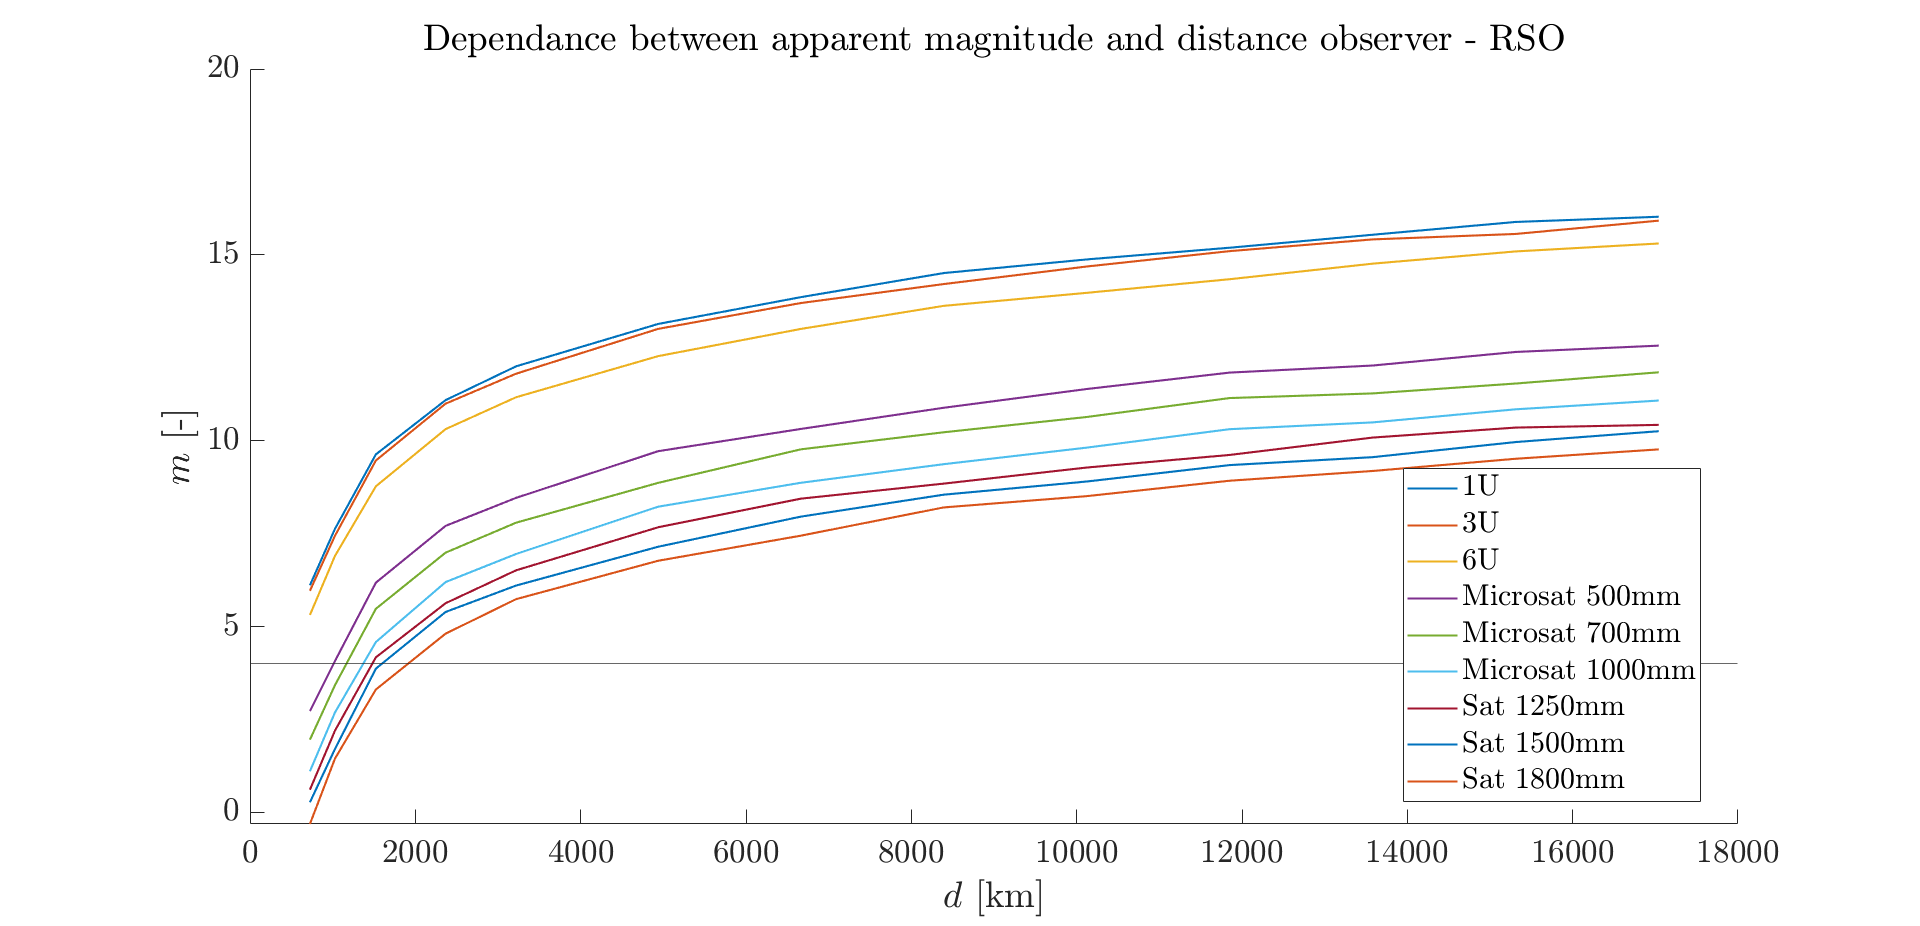
\includegraphics[width=\textwidth]{Figures/mapp-distance.png}
    \caption{}
    \label{fig:mapp-distance}
\end{figure}
\begin{figure}[H]
    \centering
    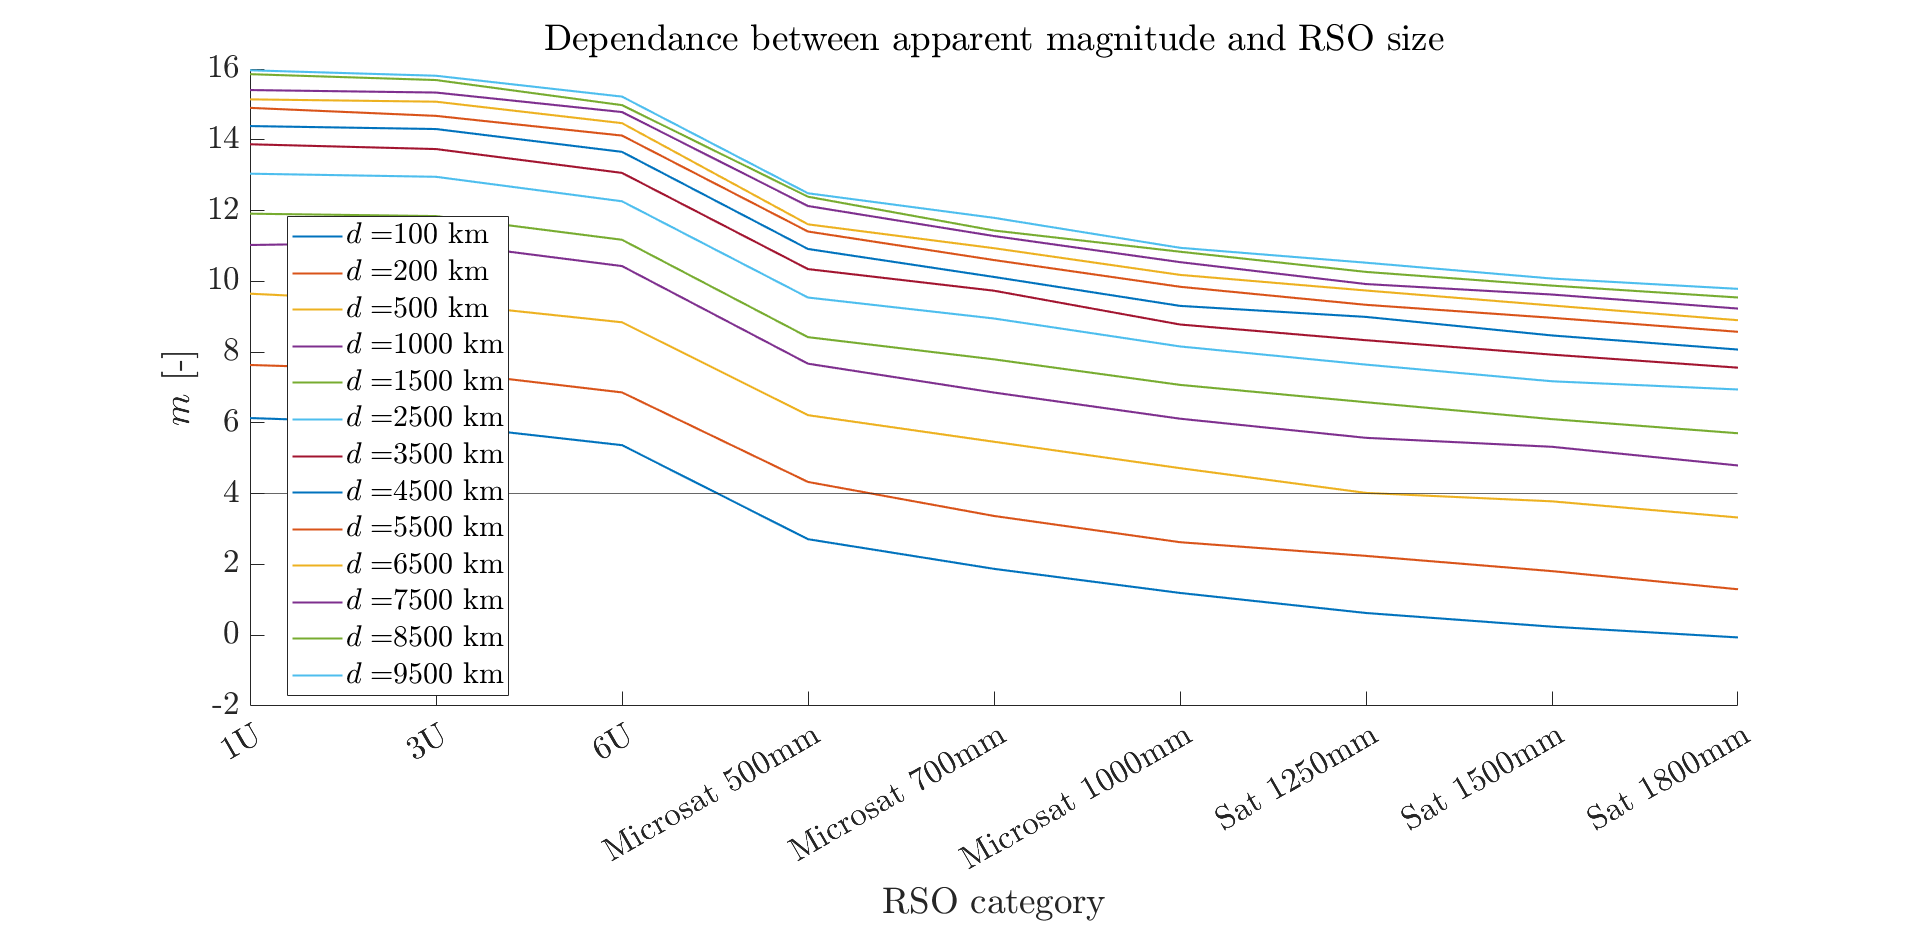
\includegraphics[width=\textwidth]{Figures/size-mapp.png}
    \caption{}
    \label{fig:mapp-size}
\end{figure} 

The apparent magnitude that the observer is able to perceive is constrained by the optical sensors employed, which will depend on factors such as the mission budget, the number of observers, and the desired constellation type. Initially, the plan is to utilize a constellation of cubesats equipped with basic tracking cameras. Following the guidelines from \cite{limmapp}, a visibility threshold has been set at $m=4$.

Returning to the examination of the previous figures, this constraint on the apparent magnitude that the observer can perceive limits a range of distances and sizes of RSOs that the satellite will be able to detect. Thus, it has been established that the observer-RSO limit distance for the sensors to detect the RSO is around $d=1000 \, \text{km}$.

\subsection{Observation windows}
On the other hand, to comprehend the influence of the Sun's position on the fraction of reflected light reaching the observer, another scan has been conducted. In this case, the observer (again with the orbital parameters outlined in \autoref{tab:paramsobs}) and the RSO are kept fixed, while the sun's location (in Earth inertial axes) is varied over the course of a year. The outcome of this procedure is depicted in \autoref{fig:angle-mapp}.

This figure shows the relation between the apparent magnitude of the RSO and $\theta$ (defined as the angle formed by the position vector of the RSO $\boldsymbol{r_{RSO}}$ and the Sun $\boldsymbol{r_{Sun}}$projeted into the ecuatorial plane).
\begin{figure}[H]
    \centering
    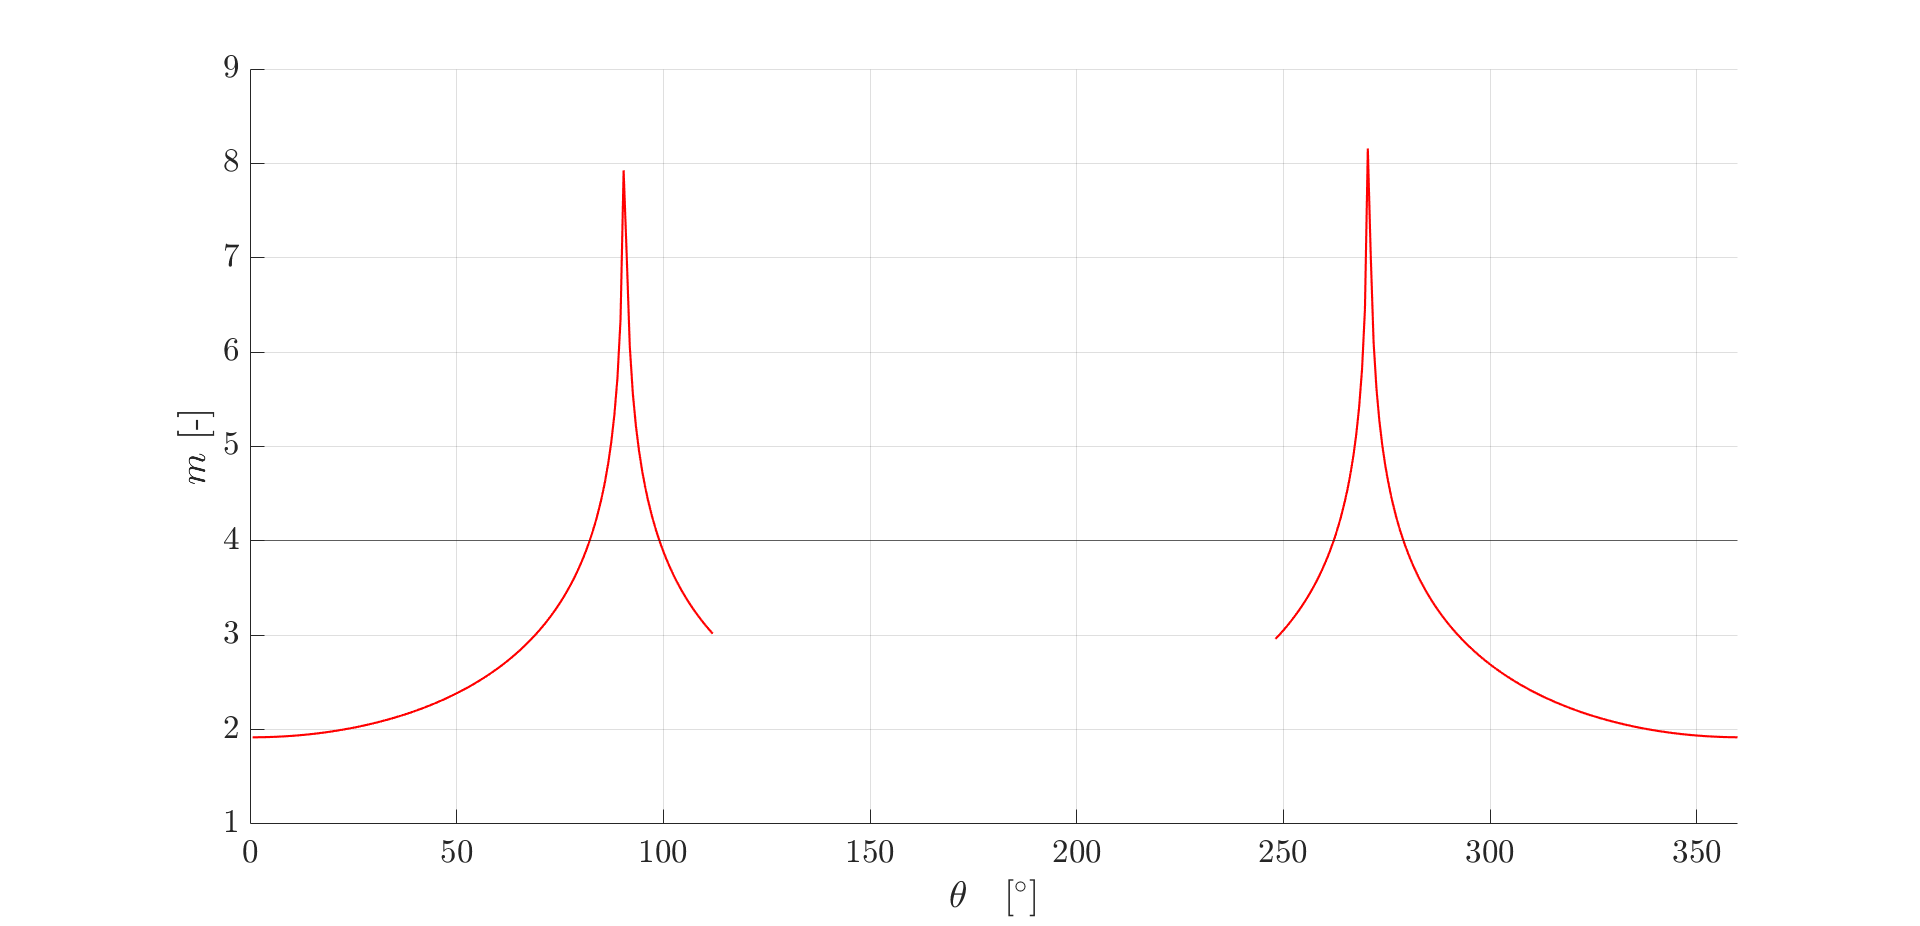
\includegraphics[width=\textwidth]{Figures/anglesunRSO-mapp.png}
    \caption{Dependance of the apparent magnitude $m$ with the position of the Sun relative to the observer.}
    \label{fig:angle-mapp}
\end{figure}

Within the \autoref{fig:angle-mapp}, it is evident that the optimal solar position occurs when $\theta$ is in close proximity to zero. However, it is fundamental to note a potential intricacy in the case of an Above-the-Horizon (ATH) coverage. Specifically, if the target aligns precisely with the sun, the resulting light curve from the target may be entirely eclipsed by the incoming sunlight. Nonetheless, for Below-the-Horizon (BTH) orbits and/or distinct inclinations, the presented outcome within this graph remains accurate. As this angle is not an input to the program, it must be translated to the date it corresponds, which can be seen in \autoref{fig:date-mapp}, where the date-defined observation window can be seen. 
\begin{figure}[H]
    \centering
    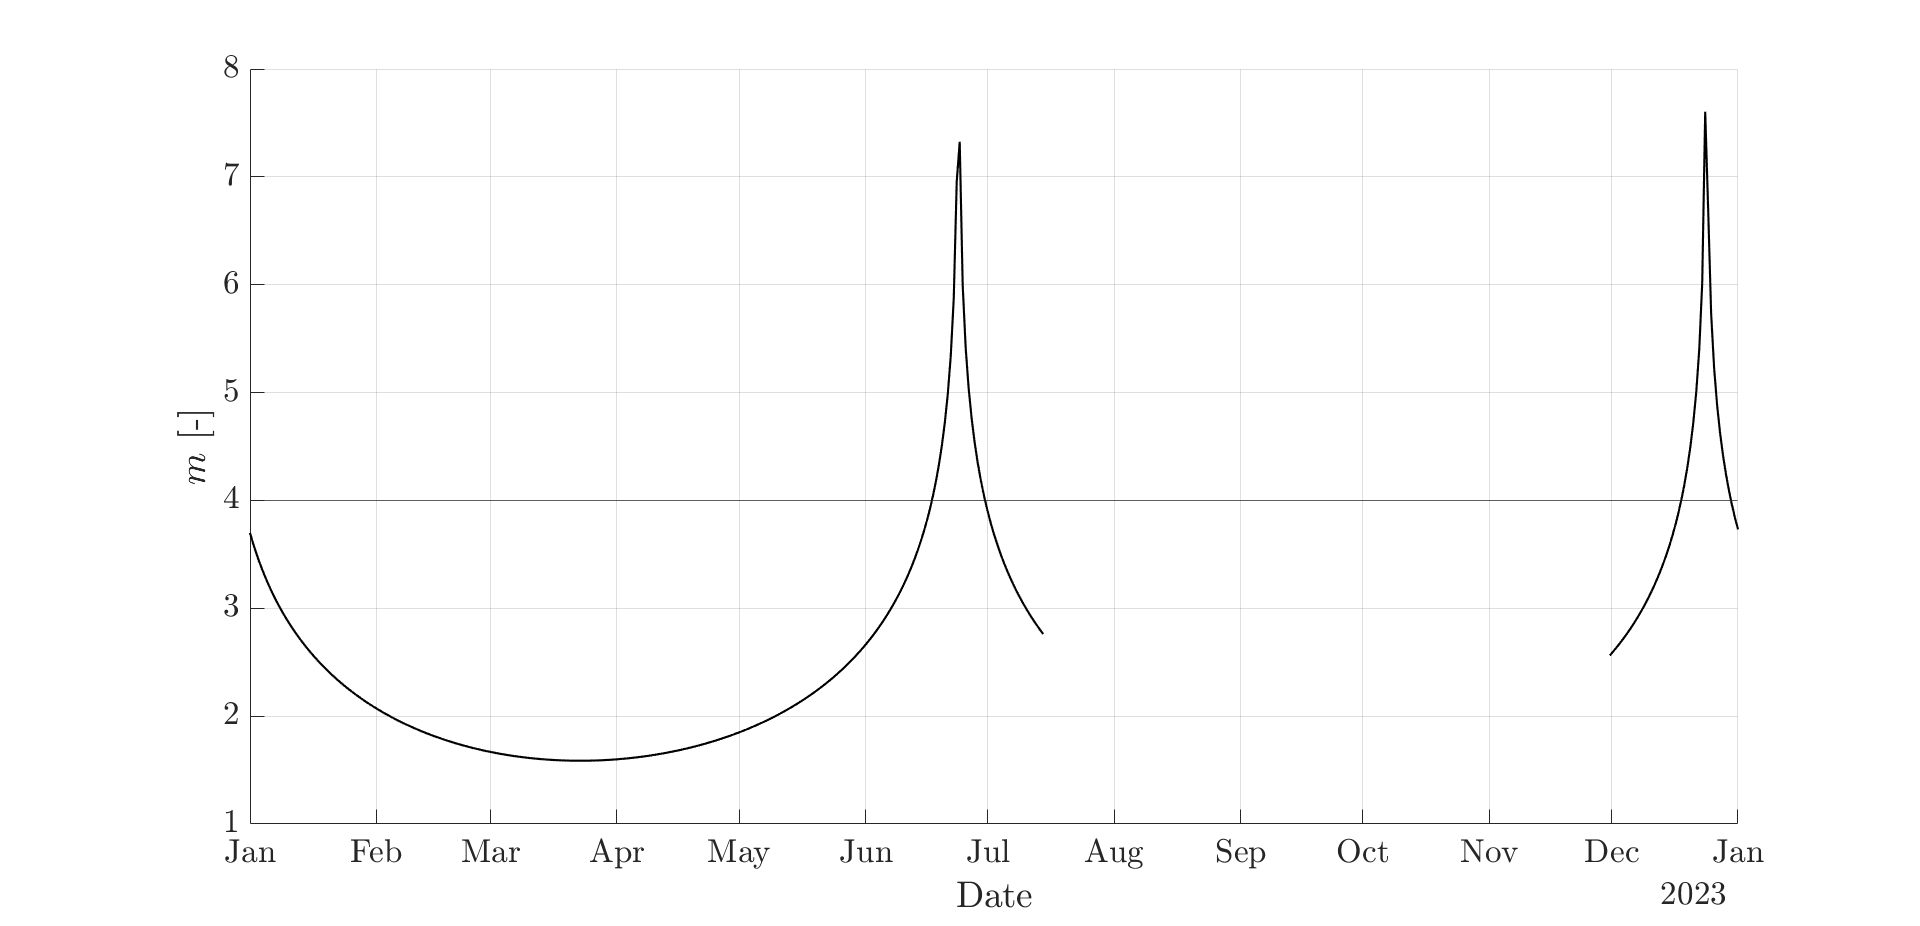
\includegraphics[width=\textwidth]{Figures/date-mapp.png}
    \caption{Dependance of the apparent magnitude $m$ with the position of the Sun in terms of date.}
    \label{fig:date-mapp}
\end{figure}

\begin{table}[H]
    \centering
    \caption{Observation window}
    \begin{tabular}{ccc}
    \toprule
     & \textbf{Start} & \textbf{End} \\
    \midrule
      $\boldsymbol{\theta}$ [$^\circ$]  & -60 & 60 \\
      \textbf{Date} & 1 January 2023 & 16 June 2023 \\
    \bottomrule
    \end{tabular}
    \label{tab:ventanas}
\end{table}

Based on these outcomes, observation windows have been delineated to subsequently conduct simulations in which the RSO falls within the field of view of the observer. 

With the information of these findings, observation windows have been meticulously defined to conduct subsequent simulations where the RSO resides within the visibility sphere of the observer. It is noteworthy that, for this parameter sweep, a distance of 300 km between the RSO and the observer has been considered, incorporating BTH coverage, and using a square-shaped satellite with a side length of 1 m.

\subsection{Visibility times}
Subsequently, multiple simulations have been executed with varying numbers of observers to assess visibility durations. For this purpose, the RSO has been fixed in an orbit with parameters outlined in \autoref{tab:paramstarget}, within the launch windows specified in \autoref{tab:ventanas}. It is essential to note that while the observation window scan was conducted for a satellite with a side length of 1 m, in this scenario, to ensure robust visibility regardless of the RSO's attitude, simulations have been conducted with a satellite measuring 1.5 m in side length. In order to obtain consistent results, the simulations were run 20 times per altitude, averaging the simulation times so that the random attitude of the RSO would not affect the visibility times. Furthermore, the number of obvservers was set to five. However, after running the simulations, the results indicated that, with the orbital positioning studied a priori, only one or at most two of the observers were able to distinguish the RSO during one orbit.

\begin{table}[H]
    \centering
    \caption{Orbital parameters of the RSO's orbit.}
    \begin{tabular}{ccc}
    \toprule
    \textbf{$a$ [km]} & \textbf{$e$ [-]} & \textbf{$i$ [$^\circ$]} \\
    \midrule
    6878 & 0 & 0.6 \\
    \bottomrule
    \end{tabular}
    \label{tab:paramstarget}
\end{table}

The obtained observation times have been illustrated in \autoref{fig:T-tvis} and dimensionless representations, relative to the total simulation time, are presented in \autoref{fig:percentages}. This approach provides a clear visualization of the fraction of the orbit covered by the observer.

\begin{figure}[H]
    \centering
    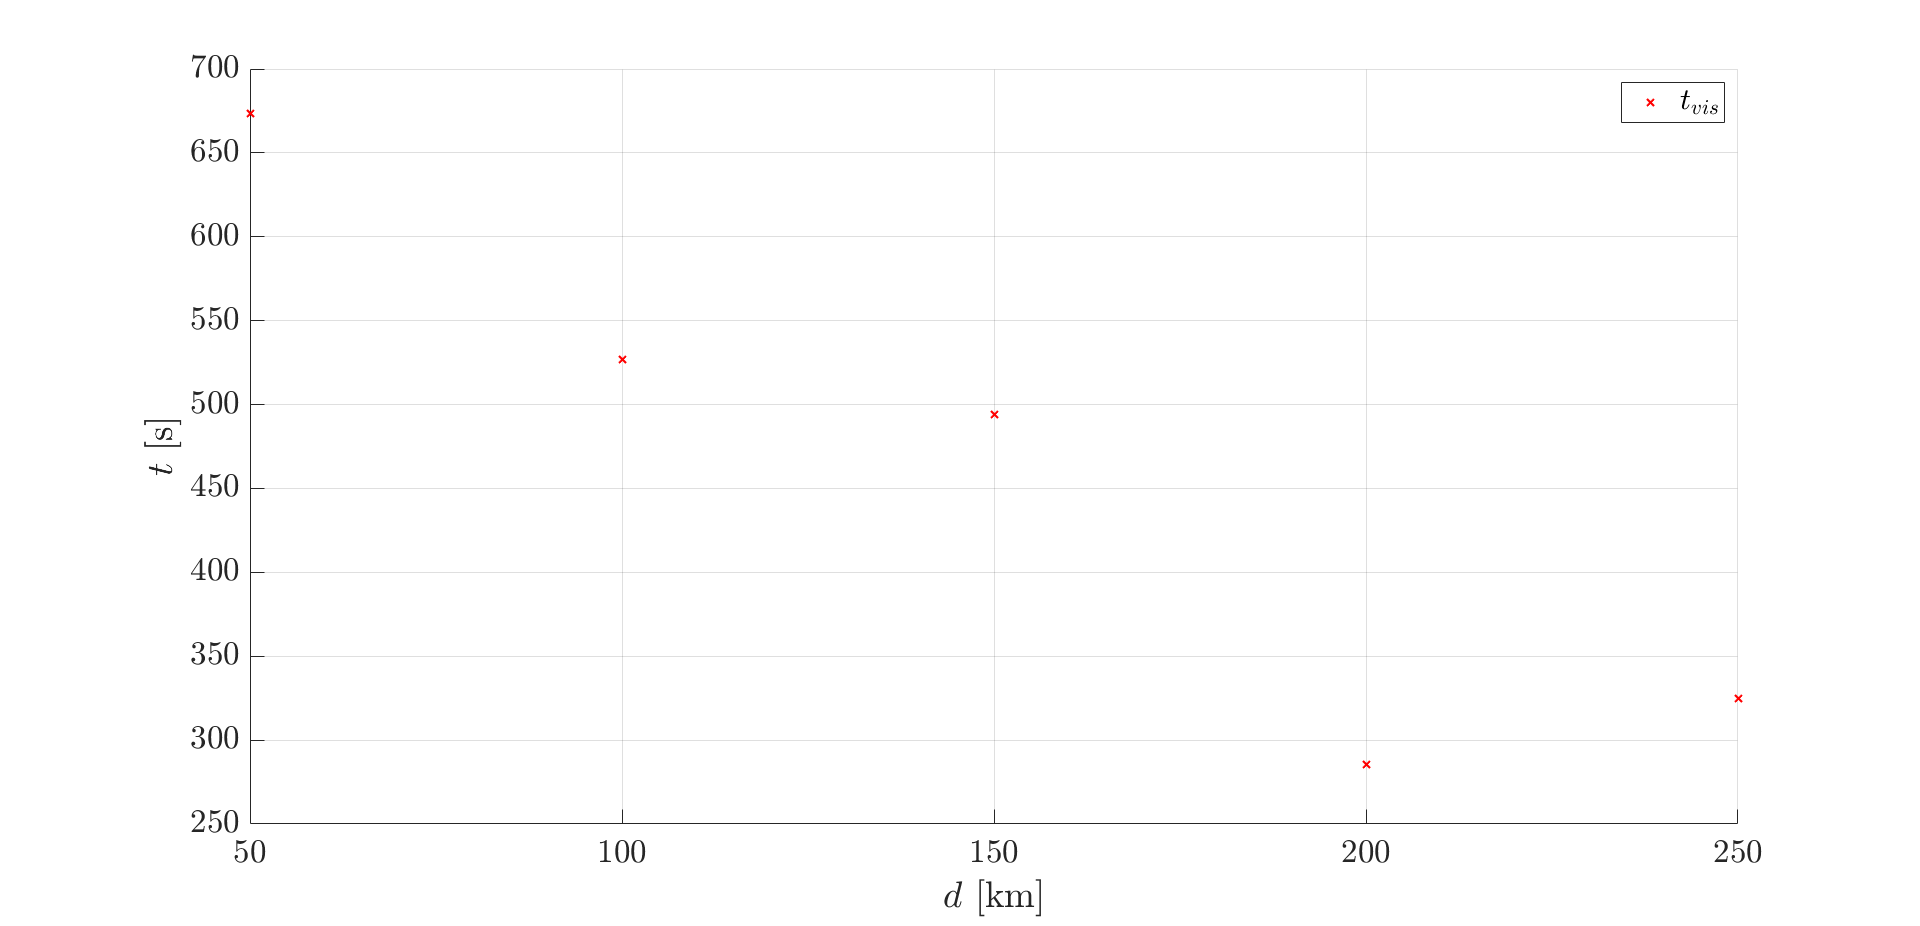
\includegraphics[width=\textwidth]{Figures/T-tvis.png}
    \caption{Dependance of the observation time with the distance between the observer and the RSO}
    \label{fig:T-tvis}
\end{figure}

\begin{figure}[H]
    \centering
    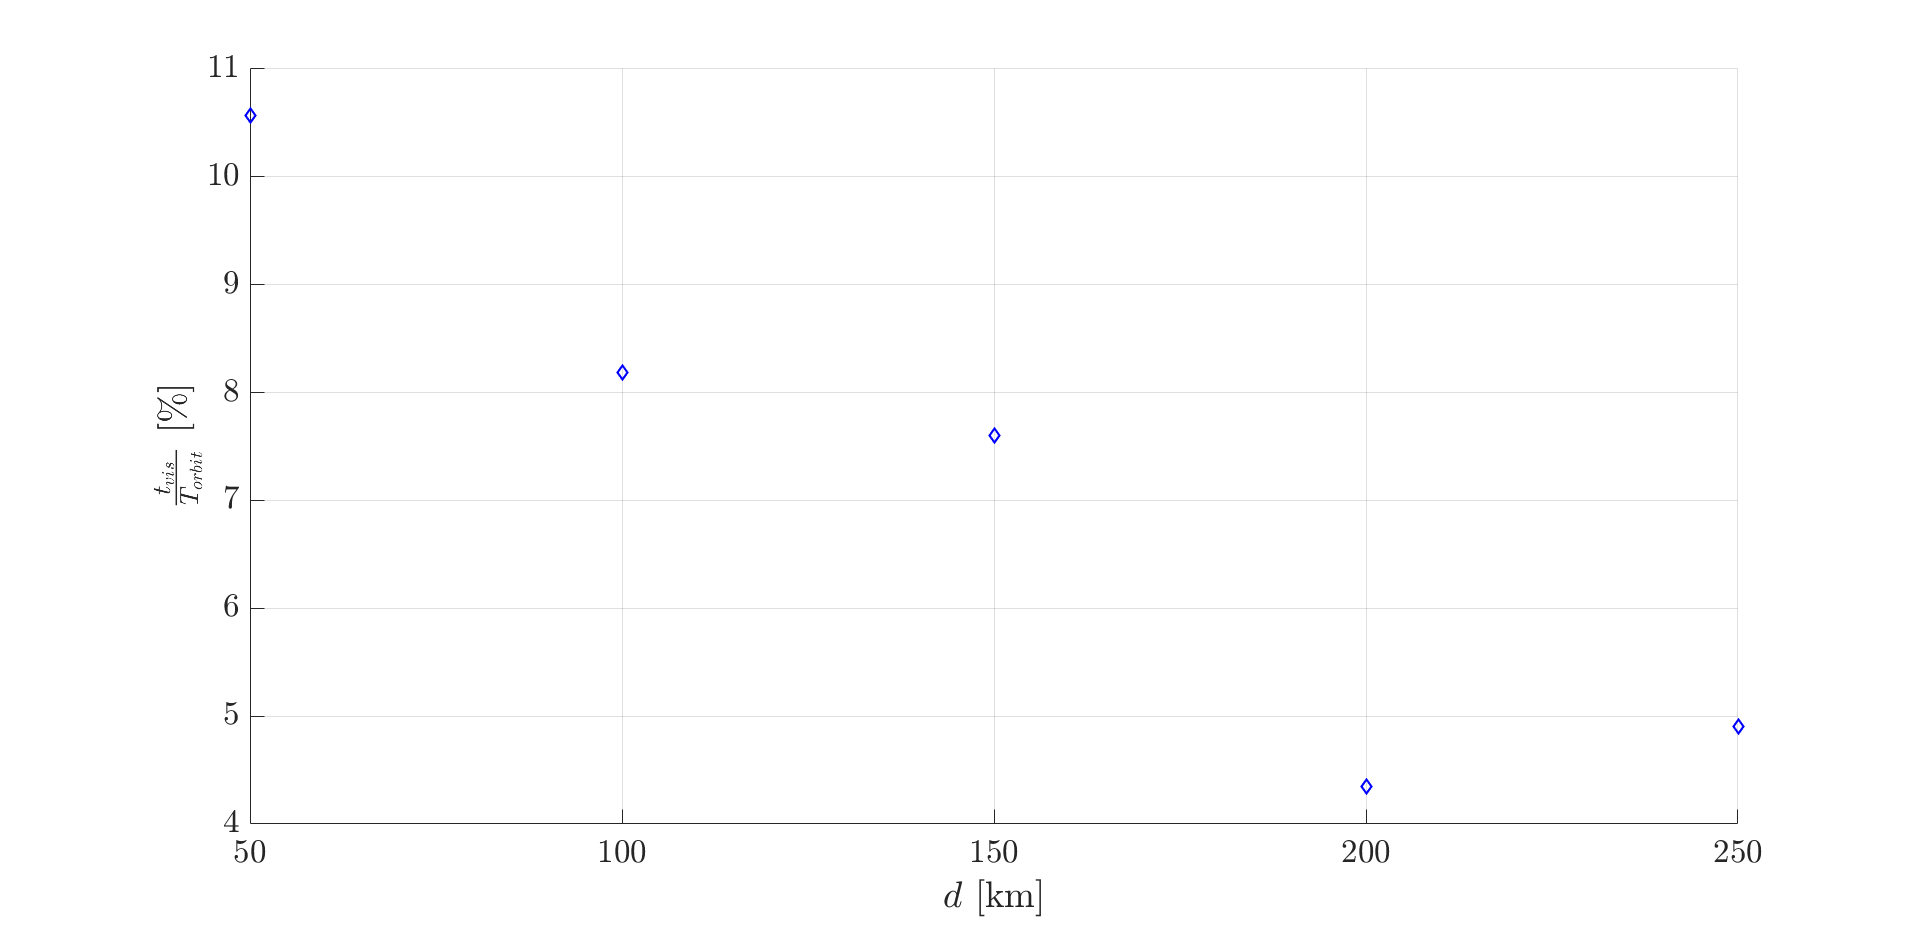
\includegraphics[width=\textwidth]{Figures/percentage-orbit.png}
    \caption{Relation between the percentage of orbit visible and the distance between the observer and the RSO}
    \label{fig:percentages}
\end{figure}

Note in Figures \ref{fig:T-tvis} and \ref{fig:percentages} that increasing the distance between the observer and the RSO decreases the duration of the observation times. However, for a distance of 250 km, the RSO enters the second observer's range of observation, thus increasing the visibility time.


\subsection{Kalman Filter Precission}
Finalmente se ha hecho un estudio de la precisión del filtro de Kalman en función del numero de observadores y del tiempo medio de visibilidad de los mismos. Para ello se han analizado los valores del error en las componentes de la posición y la velocidad para distancias de 50 y 200 km y numero de observadores de 1 y 5. En las figuras b
%%%%%%%%%%%%%%%%%%%%%%%%% Error pos vec 50-5
\begin{figure}[H]
    \centering
    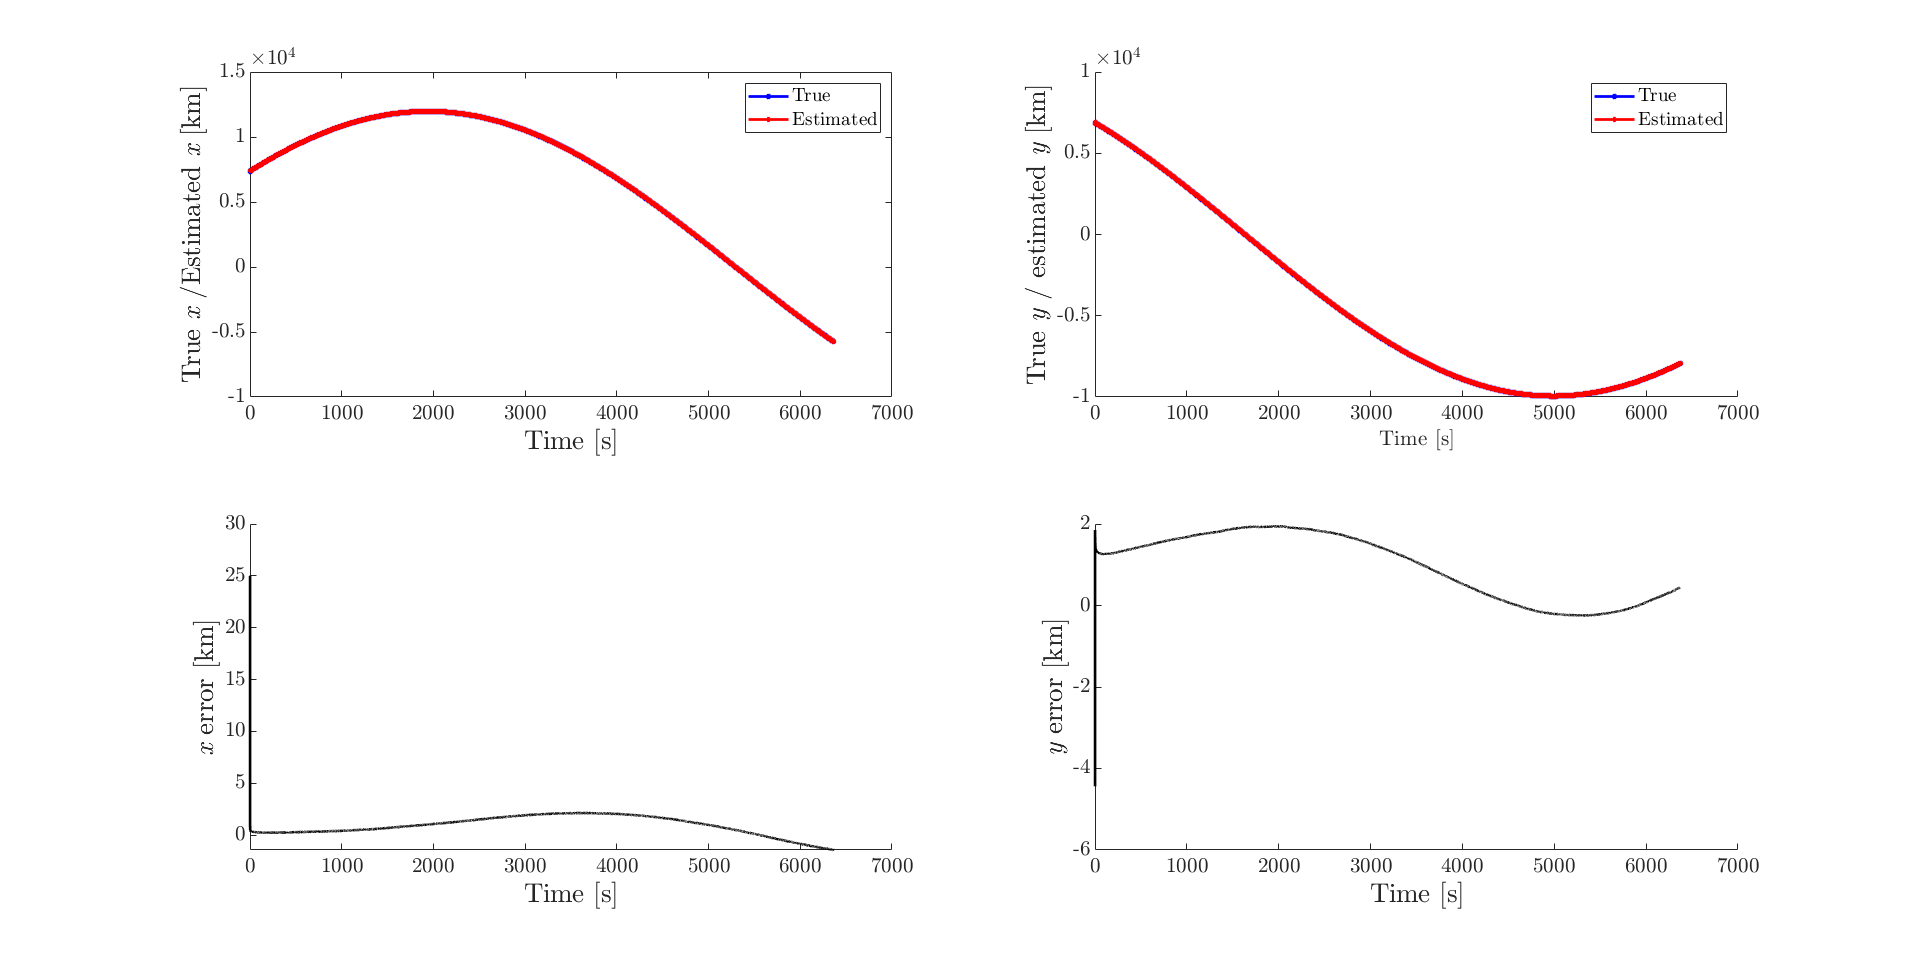
\includegraphics[width=\textwidth]{Figures/xy-error-5observers-50km.png}
    \caption{}
    \label{fig: xyerror-50-5}
\end{figure}
\begin{figure}[H]
    \centering
    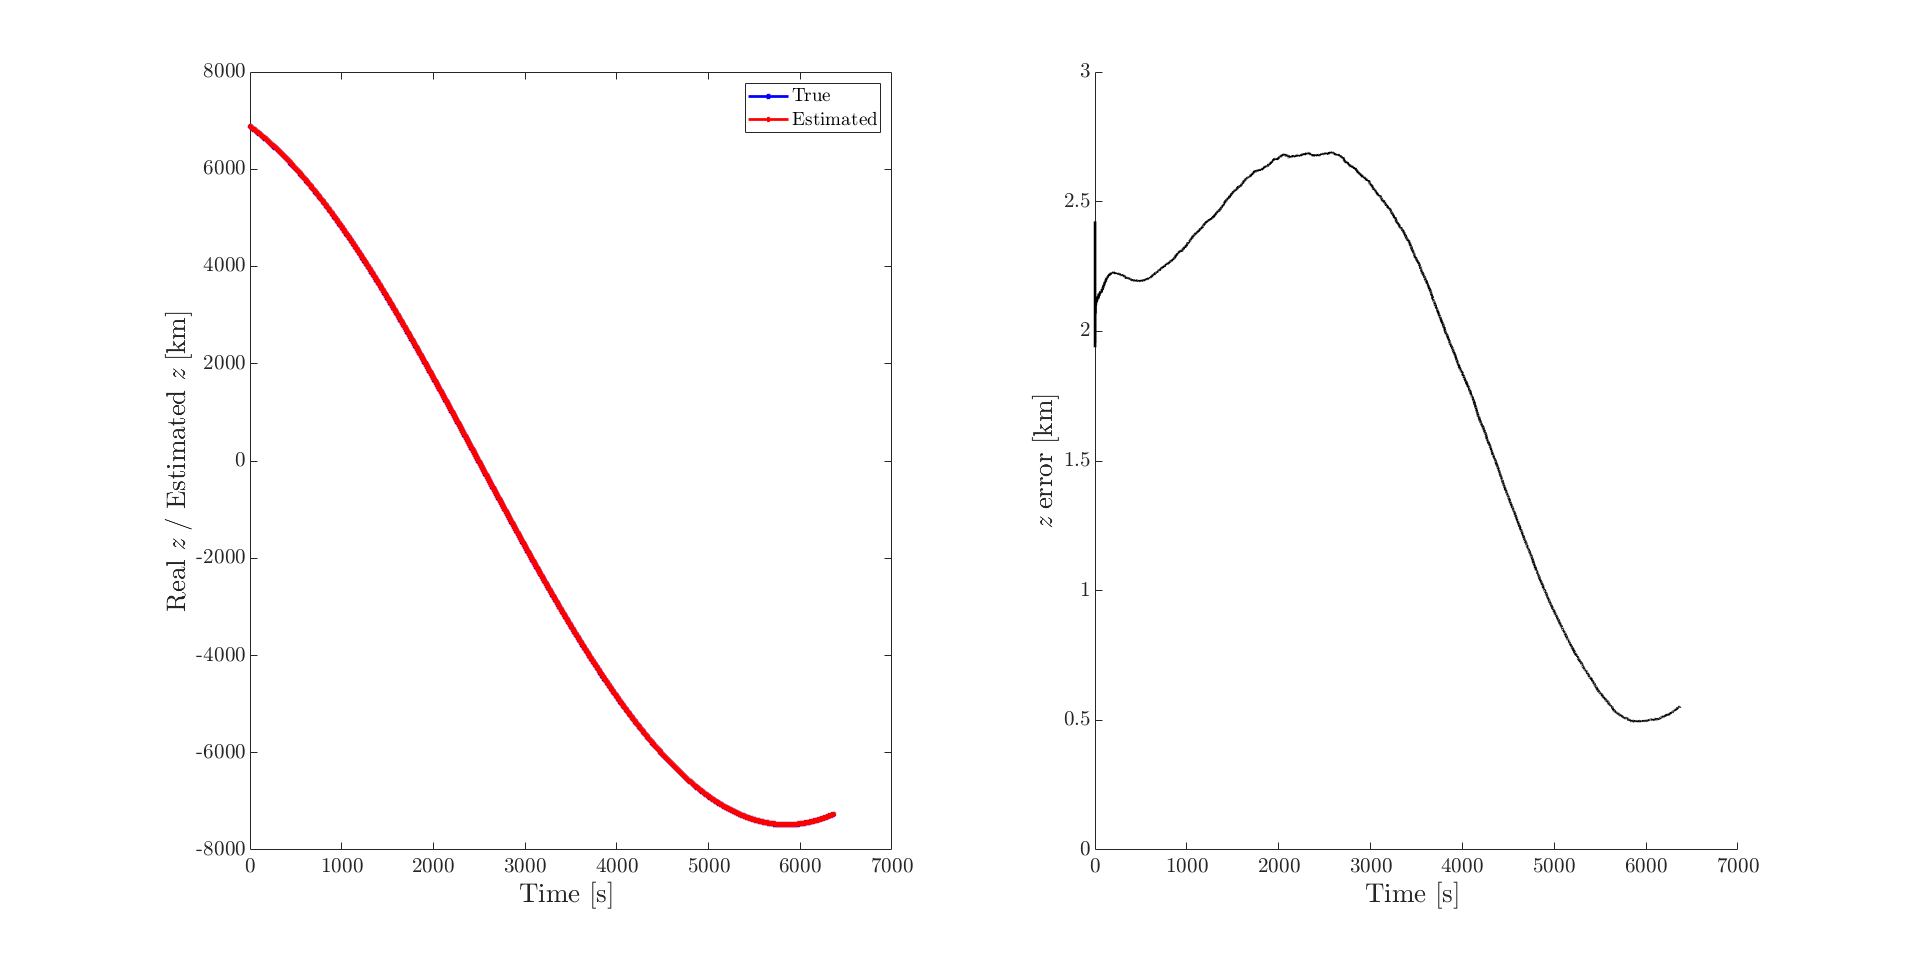
\includegraphics[width=\textwidth]{Figures/z-error-5observers-50km.png}
    \caption{}
    \label{fig: zerror-50-5}
\end{figure}
\begin{figure}[H]
    \centering
    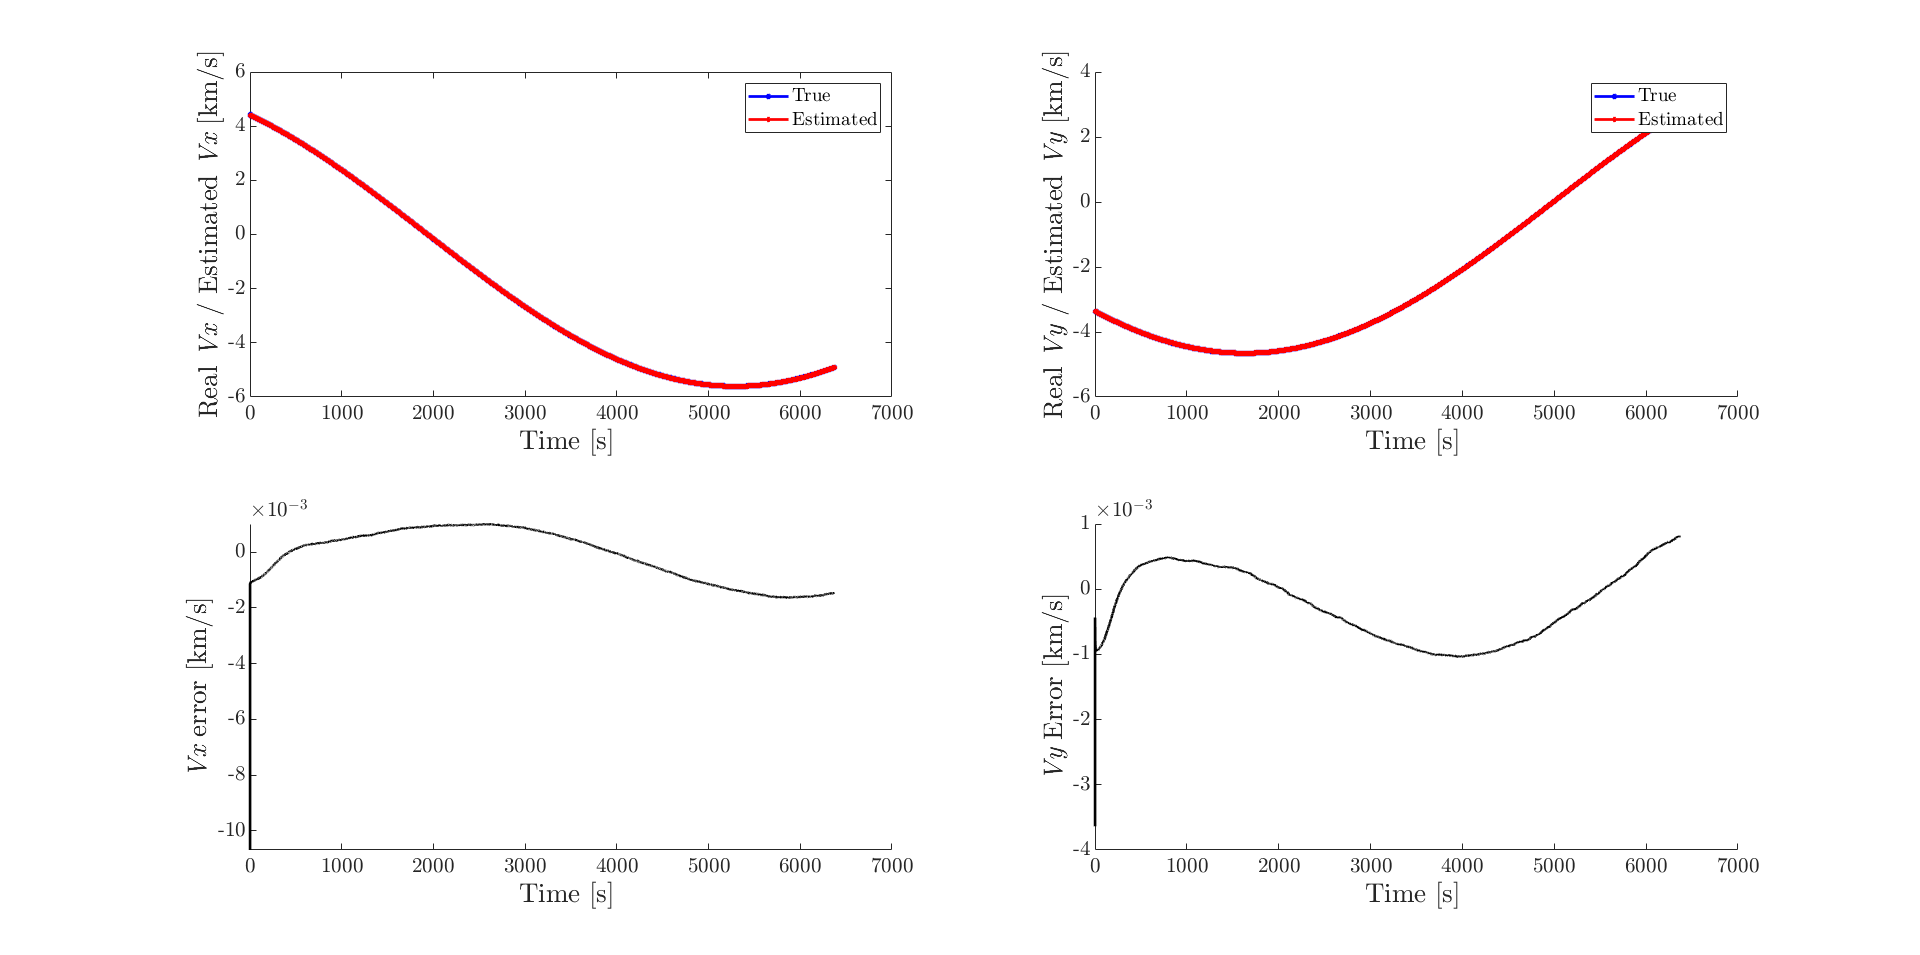
\includegraphics[width=\textwidth]{Figures/Vx-vy-error-5observers-50km.png}
    \caption{}
    \label{fig: vxyerror-50-5}
\end{figure}
\begin{figure}[H]
    \centering
    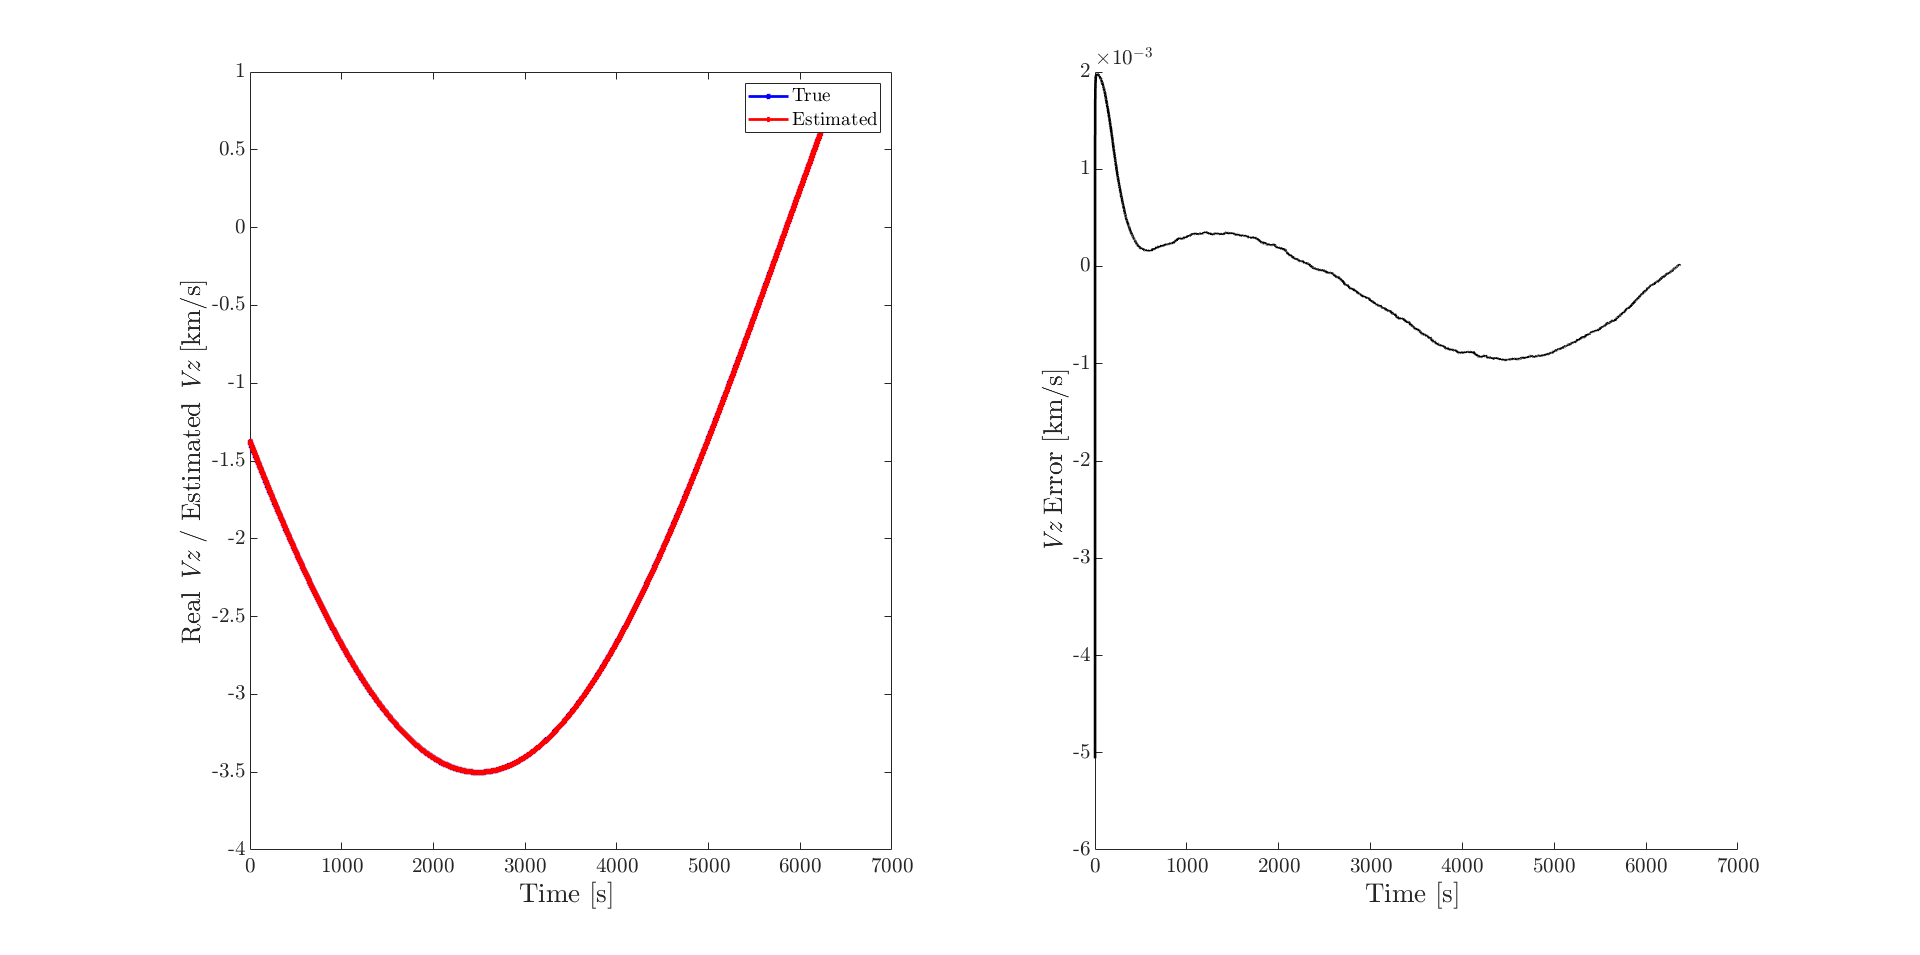
\includegraphics[width=\textwidth]{Figures/VZ_error-5observers-50km.png}
    \caption{}
    \label{fig: vzerror-50-5}
\end{figure}


%%%%%%%%%%%%%%%%%%%%%%%%% Error pos vec 250-5
\begin{figure}[H]
    \centering
    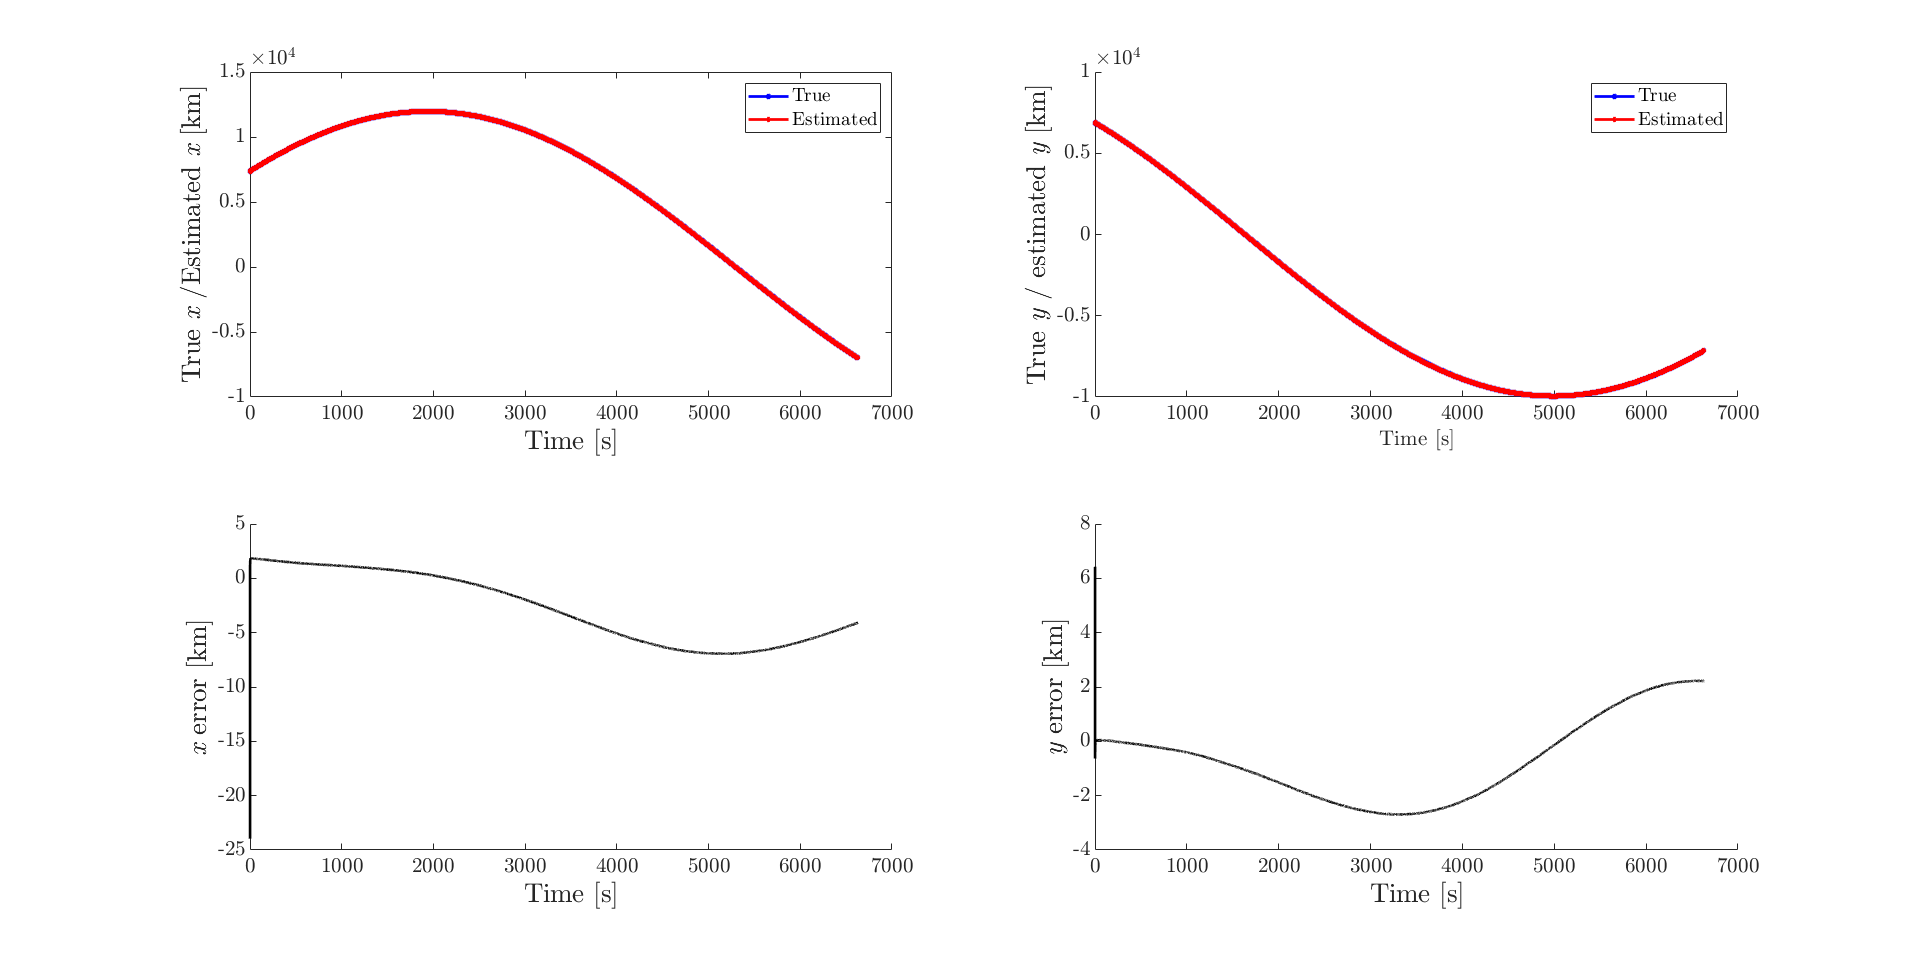
\includegraphics[width=\textwidth]{Figures/xy-error-5observers-250km.png}
    \caption{}
    \label{fig: xyerror-250-5}
\end{figure}
\begin{figure}[H]
    \centering
    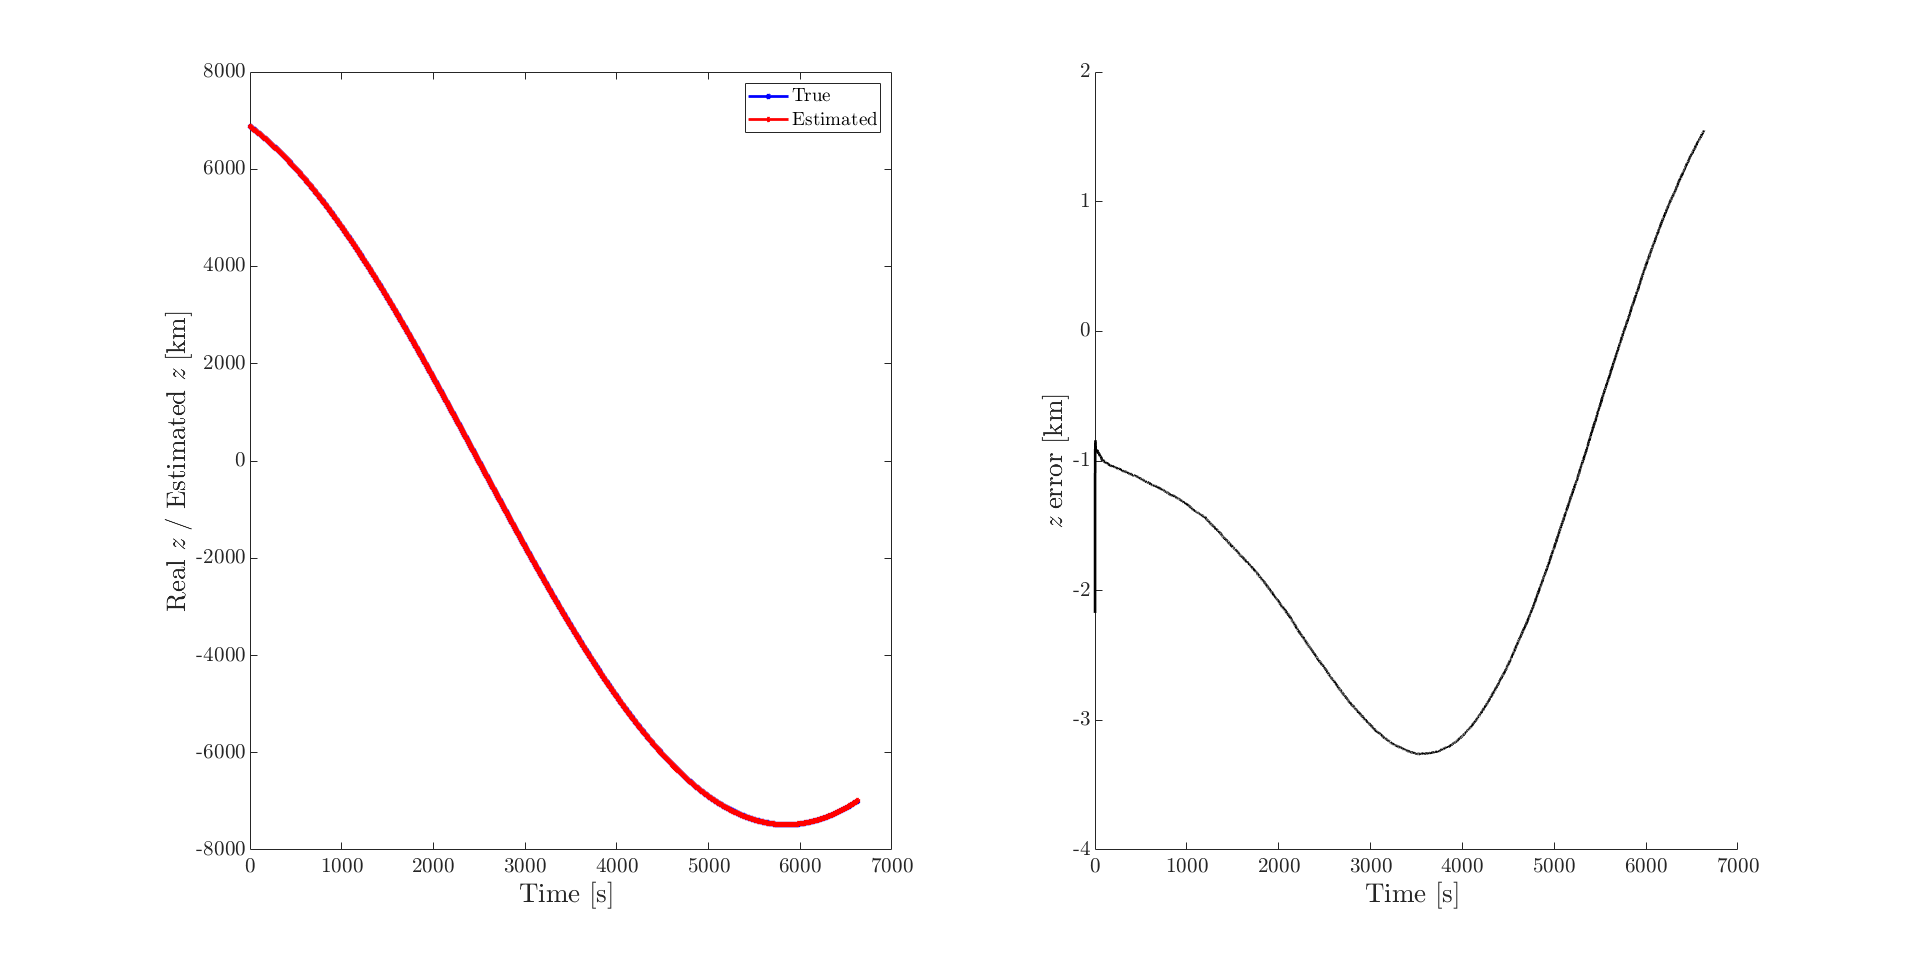
\includegraphics[width=\textwidth]{Figures/z-error-5observers-250km.png}
    \caption{}
    \label{fig: zerror-250-5}
\end{figure}
\begin{figure}[H]
    \centering
    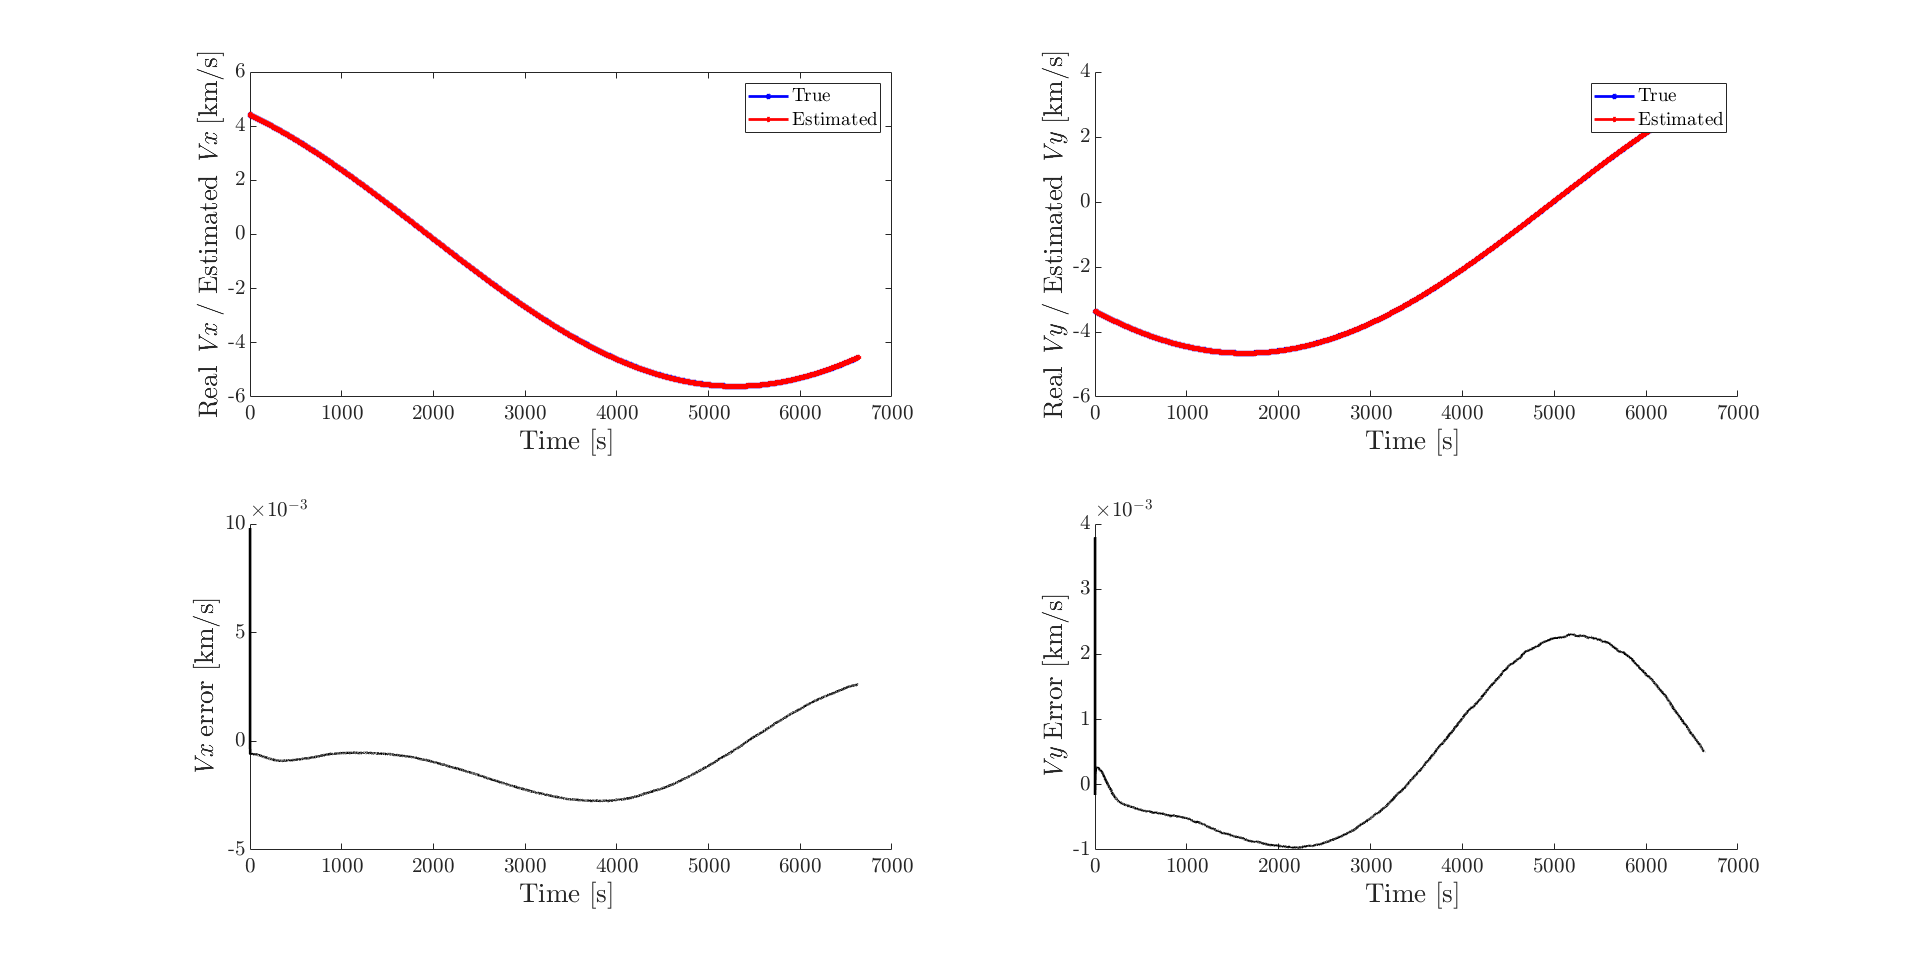
\includegraphics[width=\textwidth]{Figures/Vx-vy-error-5observers-250km.png}
    \caption{}
    \label{fig: vxyerror-250-5}
\end{figure}
\begin{figure}[H]
    \centering
    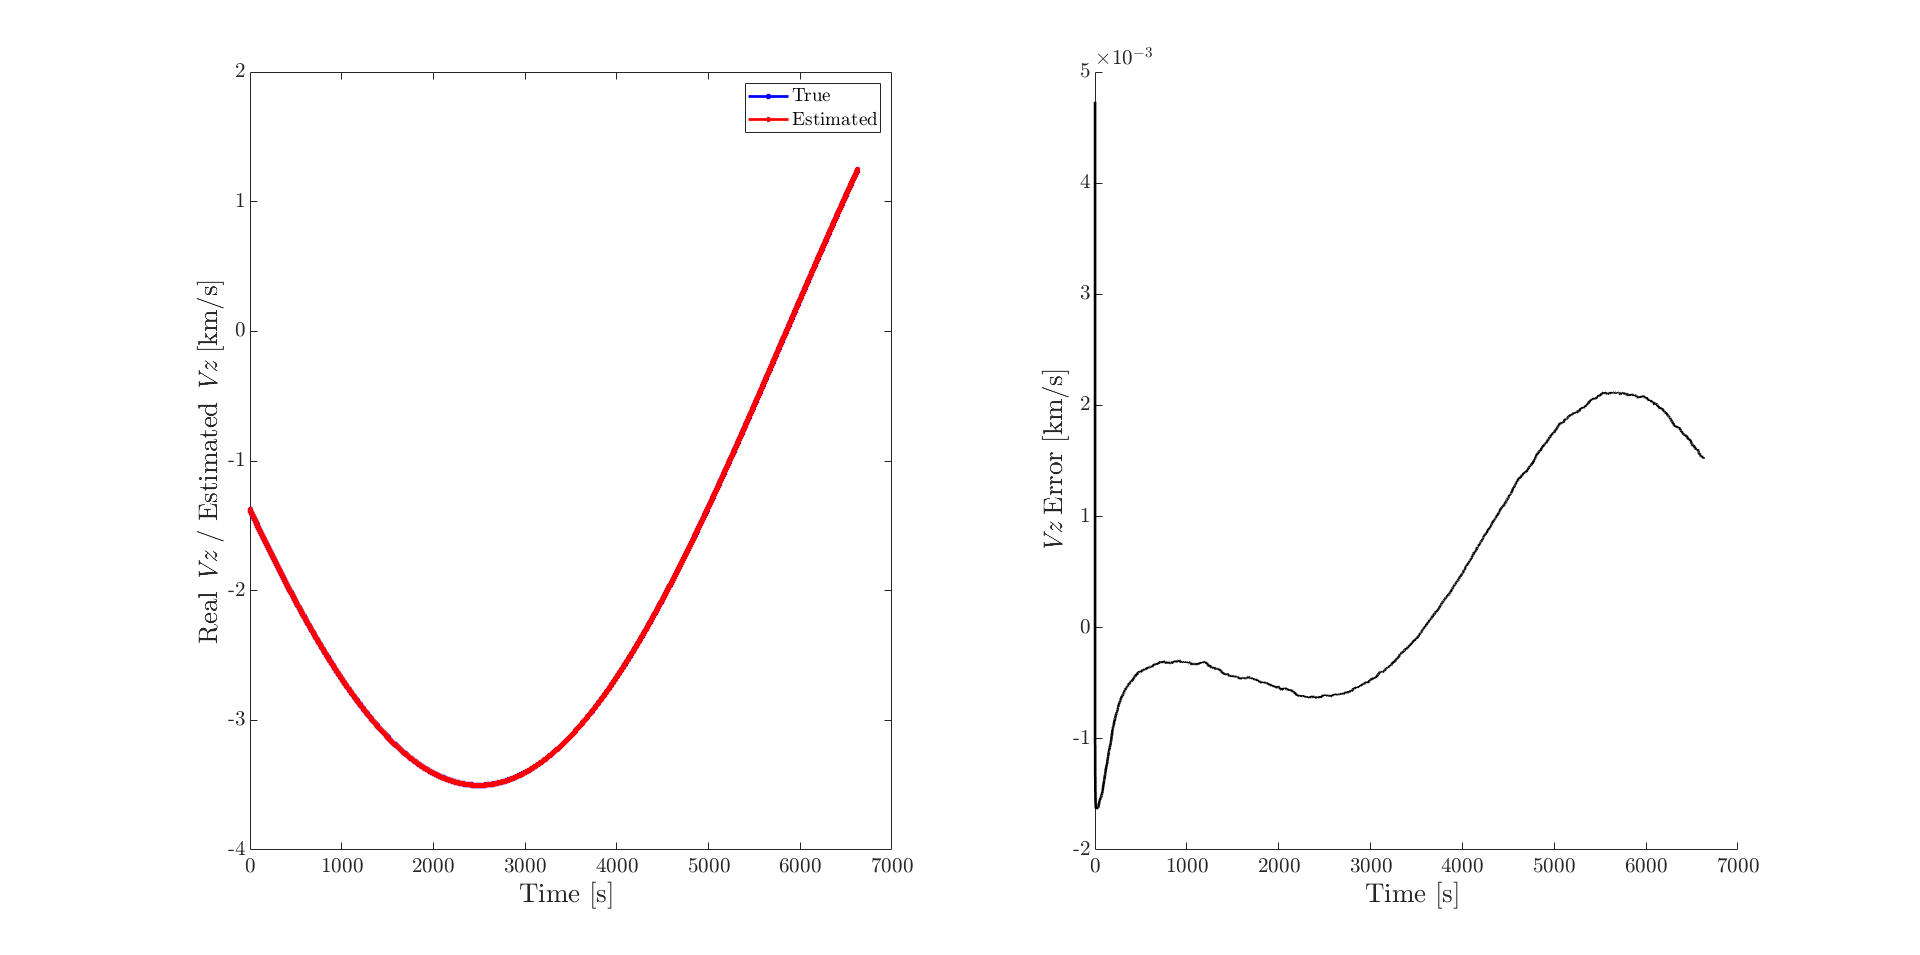
\includegraphics[width=\textwidth]{Figures/VZ_error-5observers-250km.png}
    \caption{}
    \label{fig: vzerror-250-5}
\end{figure}


%%%%%%%%%%%%%%%%%%%%%%%%% Error pos vec 50-1
\begin{figure}[H]
    \centering
    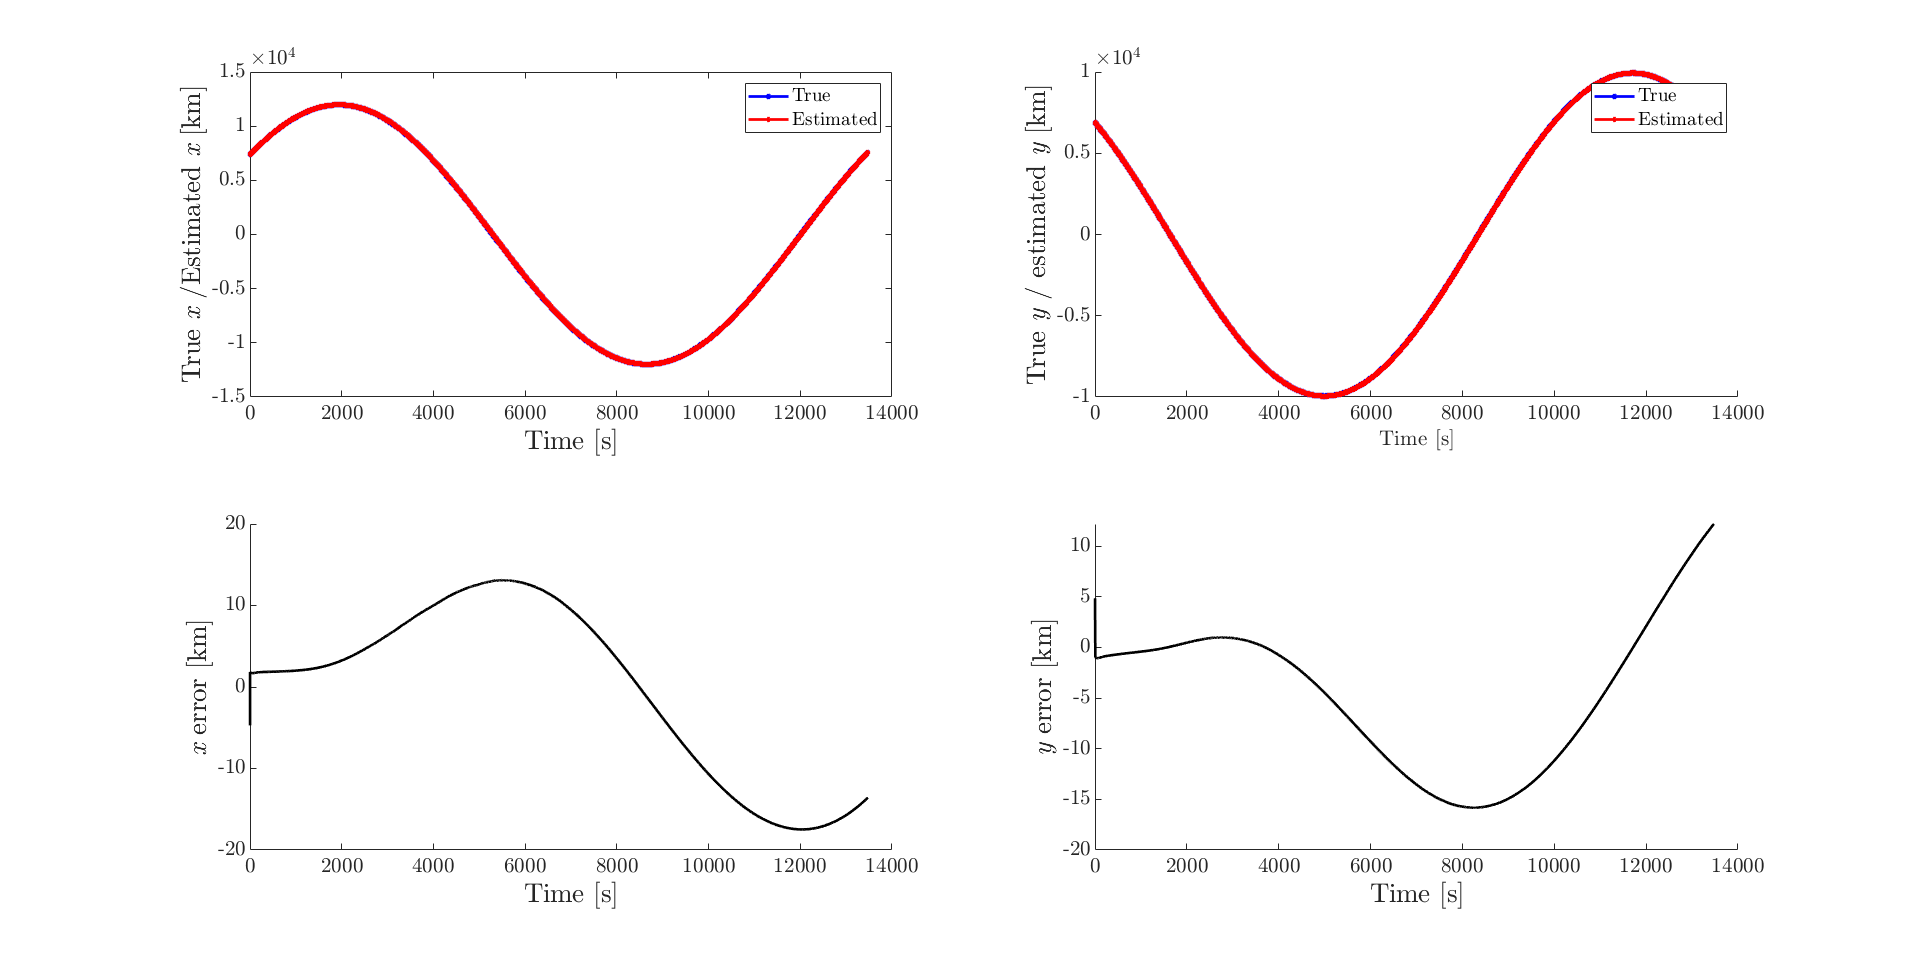
\includegraphics[width=\textwidth]{Figures/xy-error-50km-1obs.png}
    \caption{}
    \label{fig: xyerror-50-1}
\end{figure}
\begin{figure}[H]
    \centering
    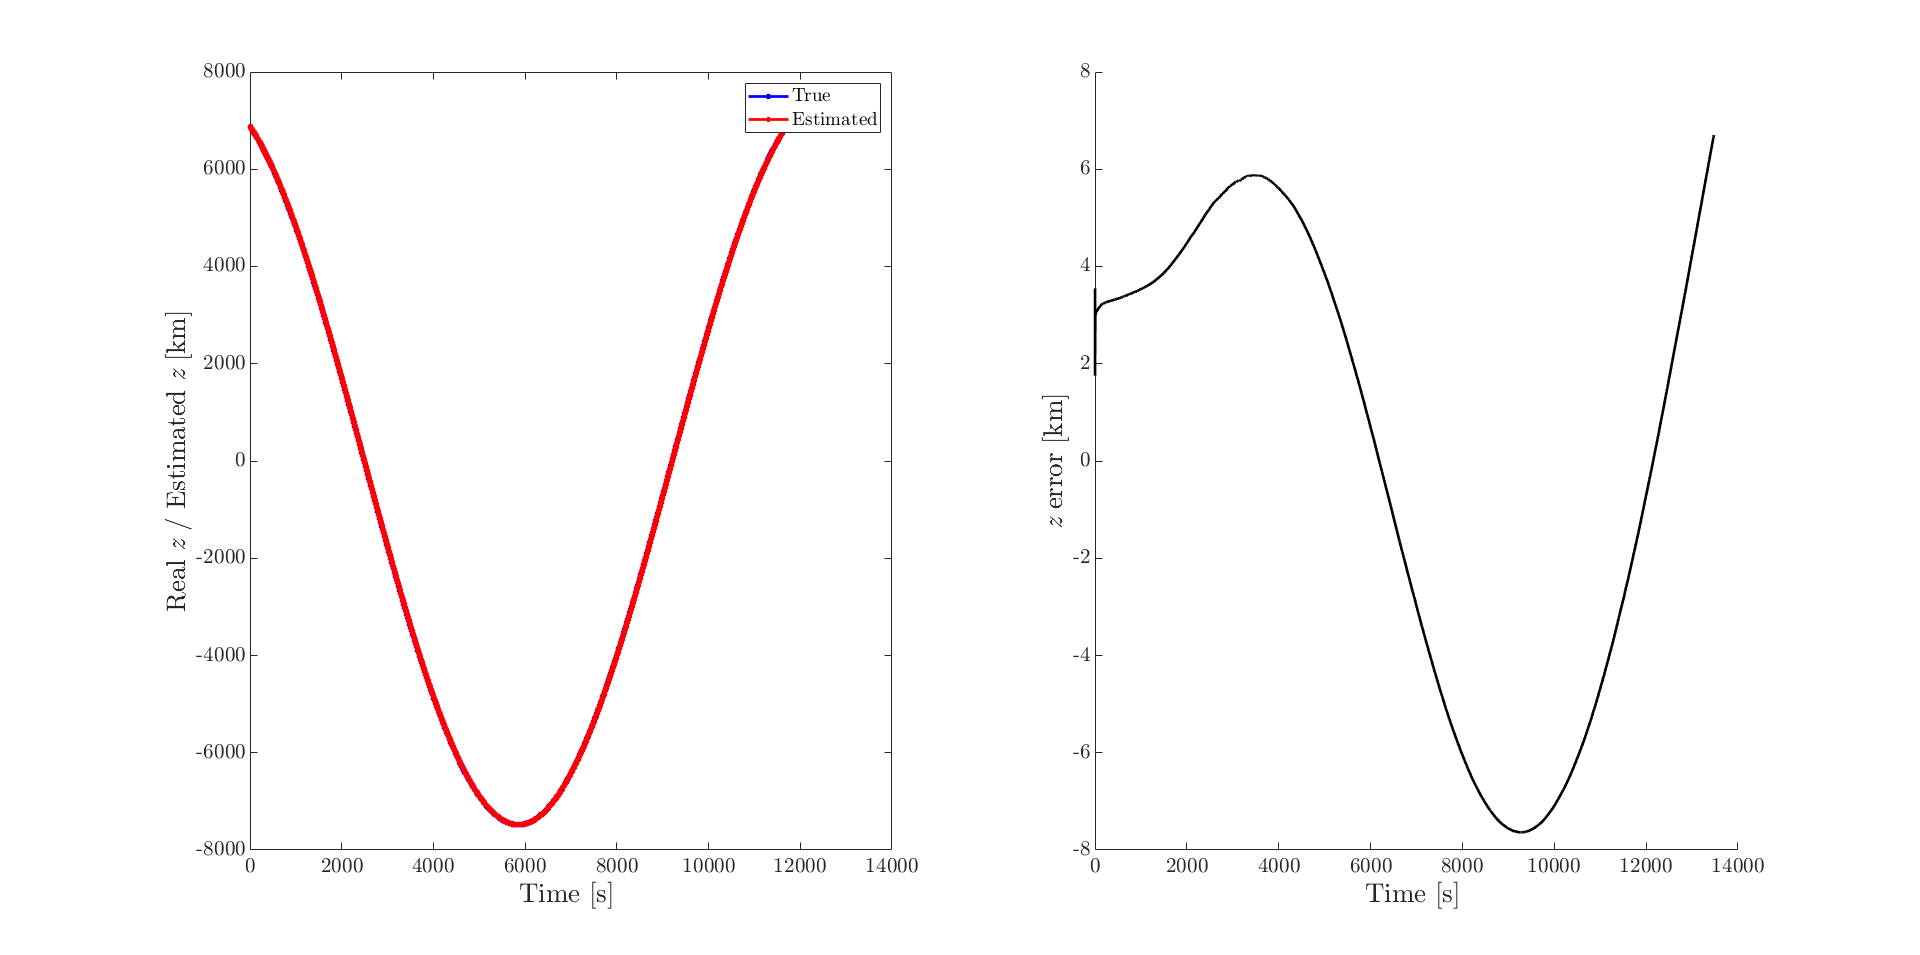
\includegraphics[width=\textwidth]{Figures/z-error-50km-1obs.png}
    \caption{}
    \label{fig: zerror-50-1}
\end{figure}
\begin{figure}[H]
    \centering
    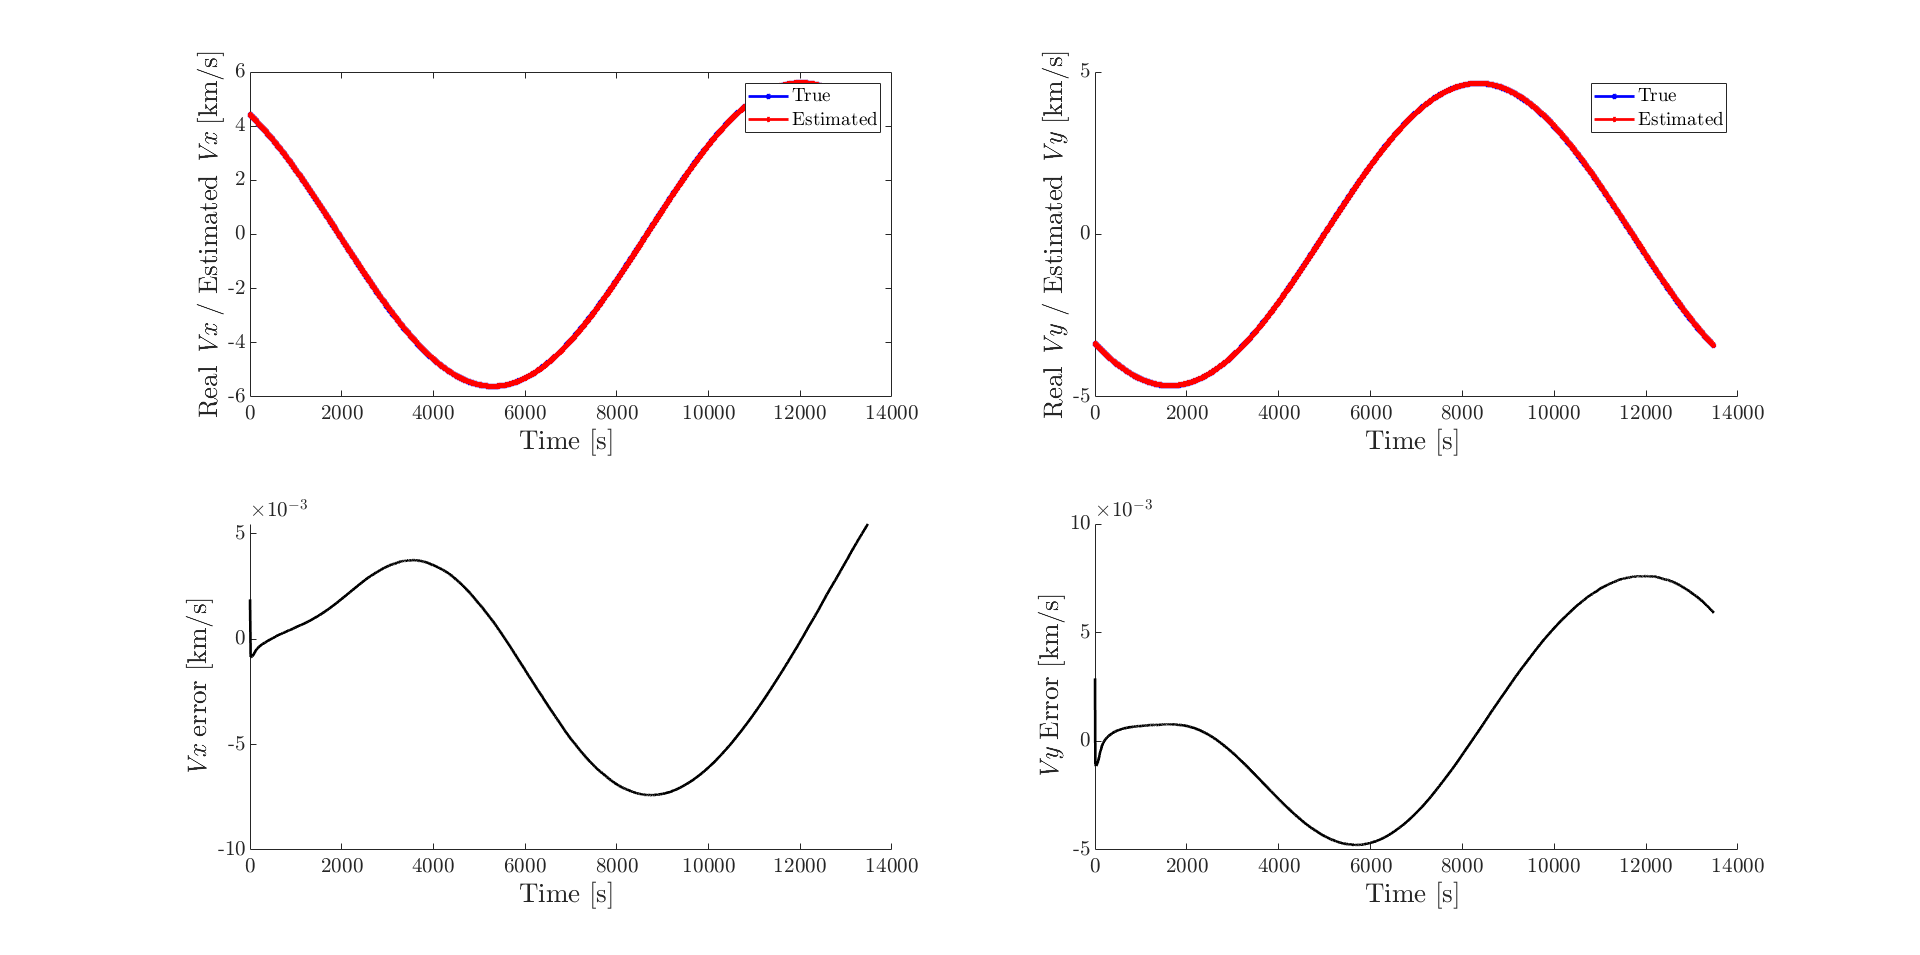
\includegraphics[width=\textwidth]{Figures/Vx-vy-error-50km-1obs.png}
    \caption{}
    \label{fig: vxyerror-50-1}
\end{figure}
\begin{figure}[H]
    \centering
    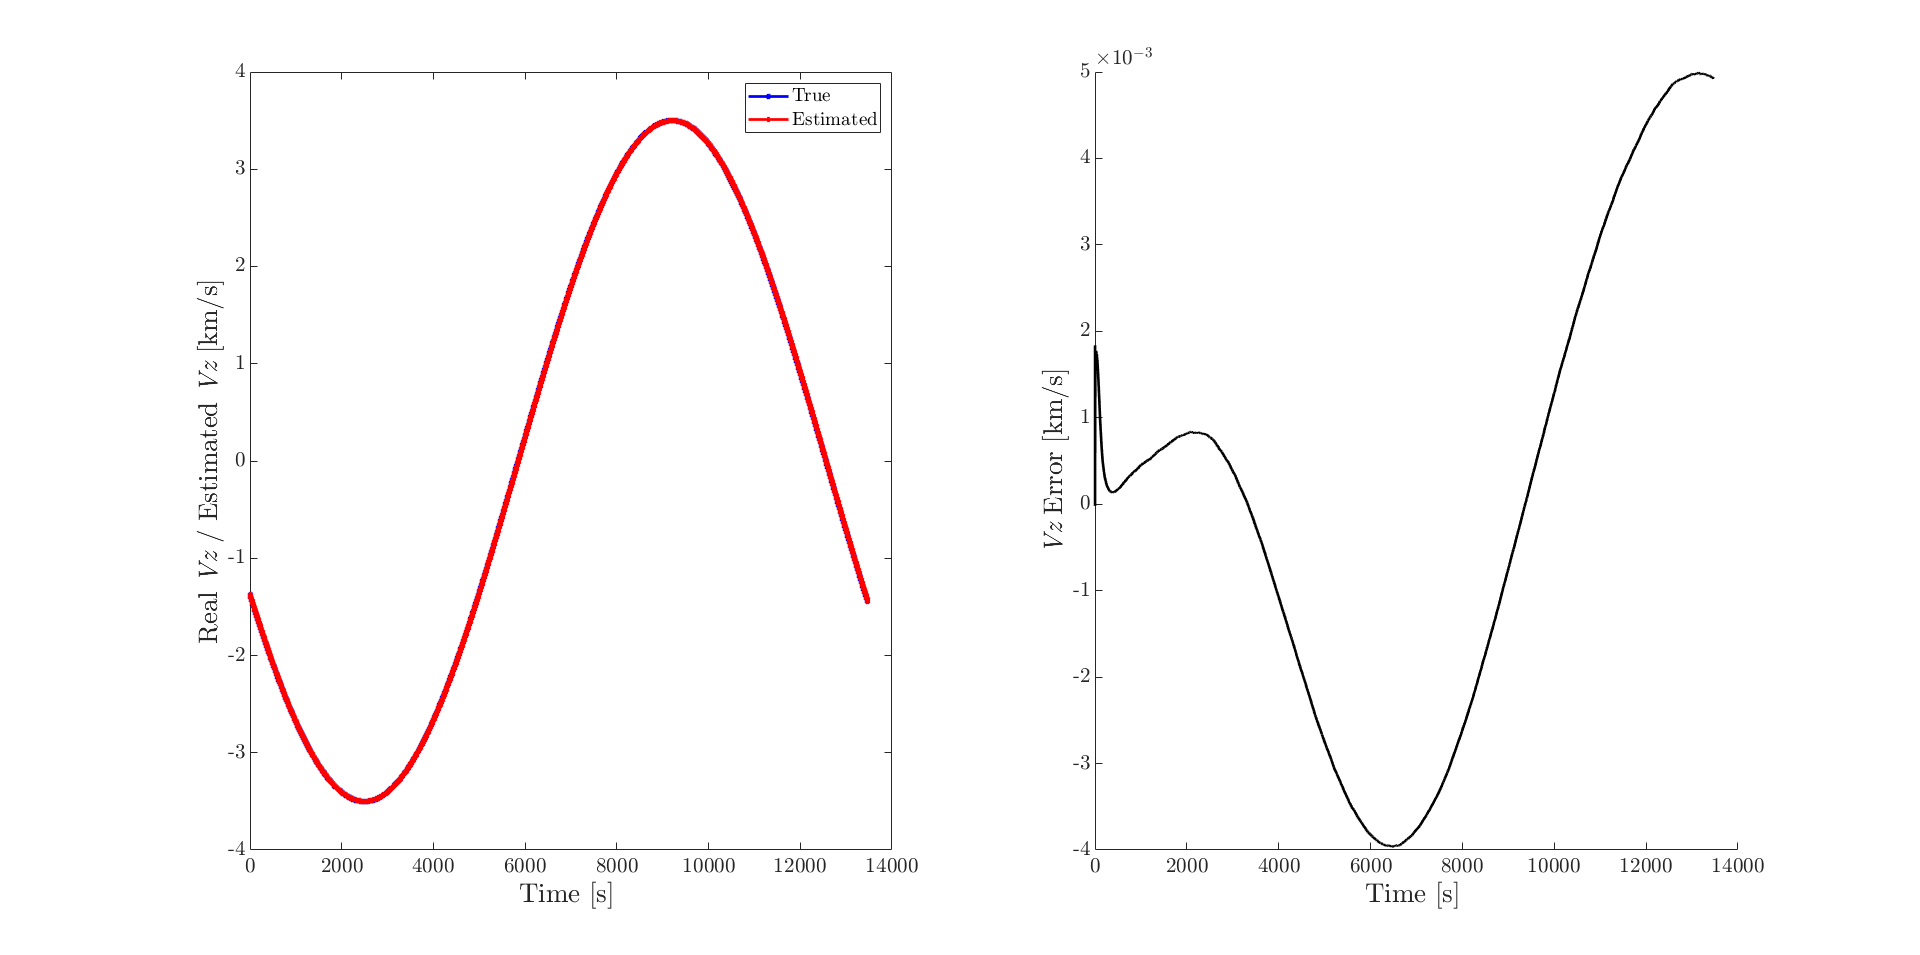
\includegraphics[width=\textwidth]{Figures/VZ_error-50km-1obs.png}
    \caption{}
    \label{fig: vzerror-50-1}
\end{figure}


%%%%%%%%%%%%%%%%%%%%%%%%% Error pos vec 250-5
\begin{figure}[H]
    \centering
    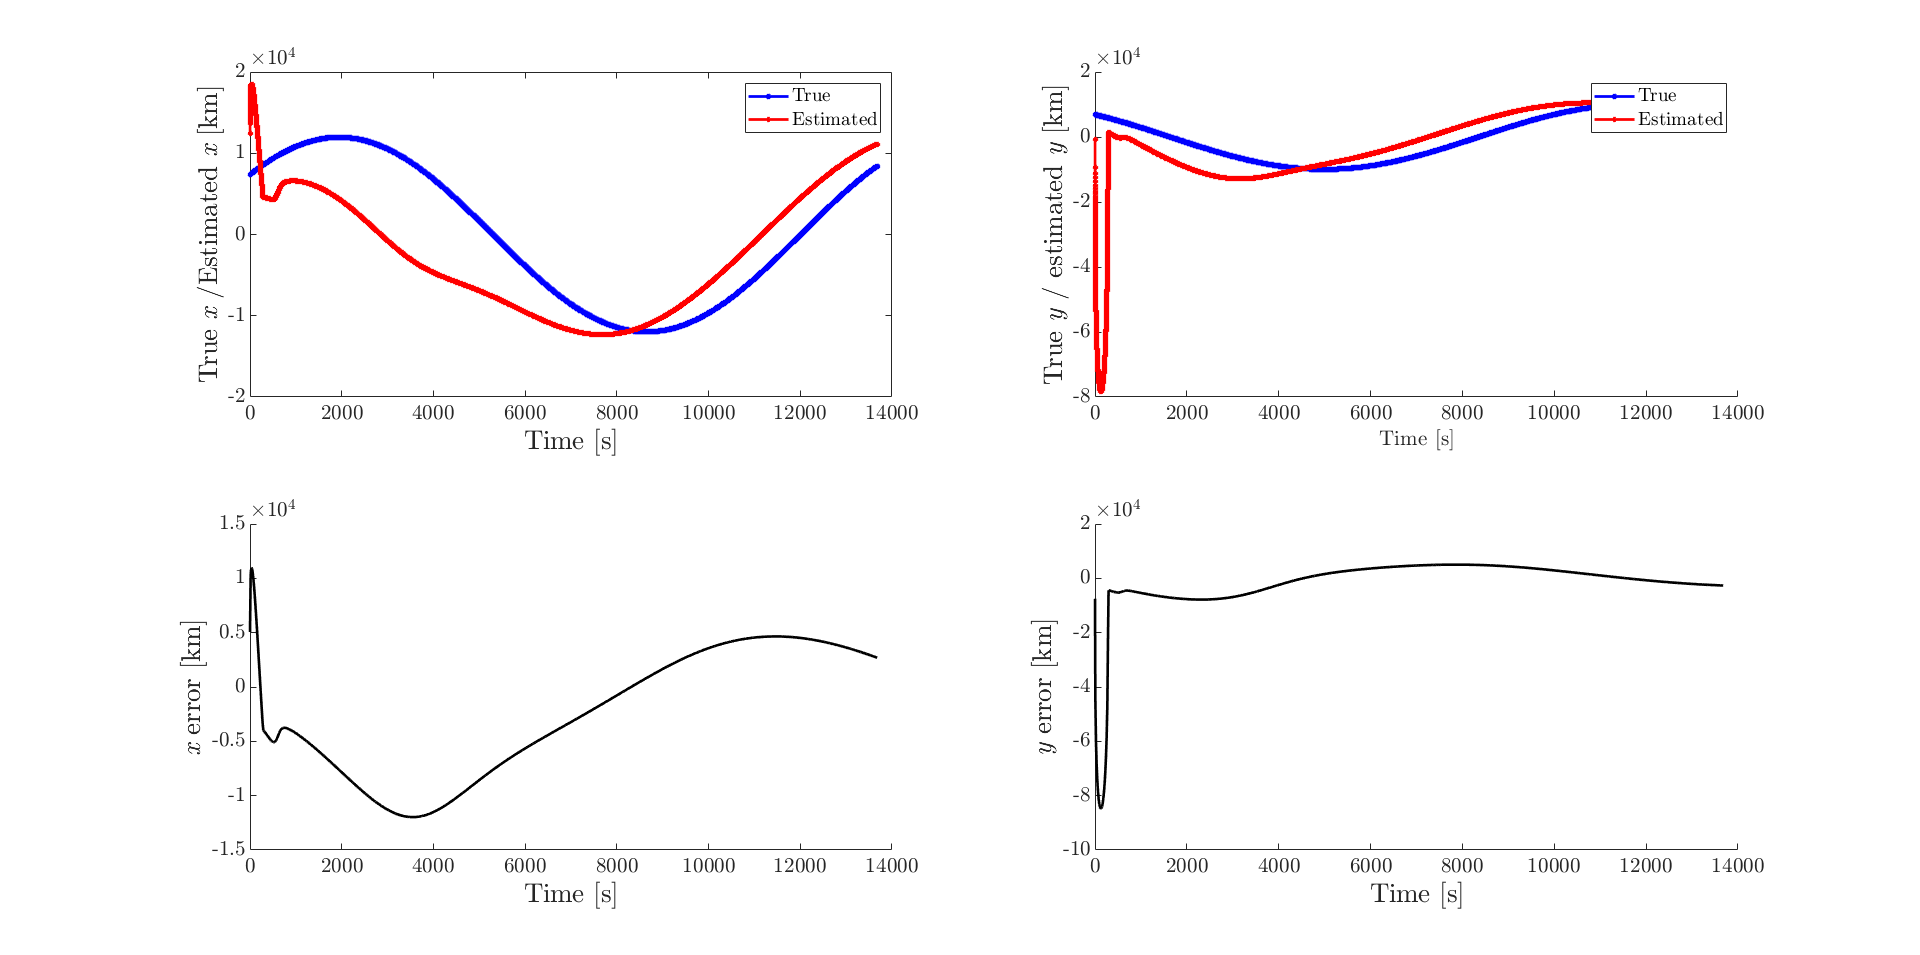
\includegraphics[width=\textwidth]{Figures/xy-error-1observers-250km.png}
    \caption{}
    \label{fig: xyerror-250-1}
\end{figure}
\begin{figure}[H]
    \centering
    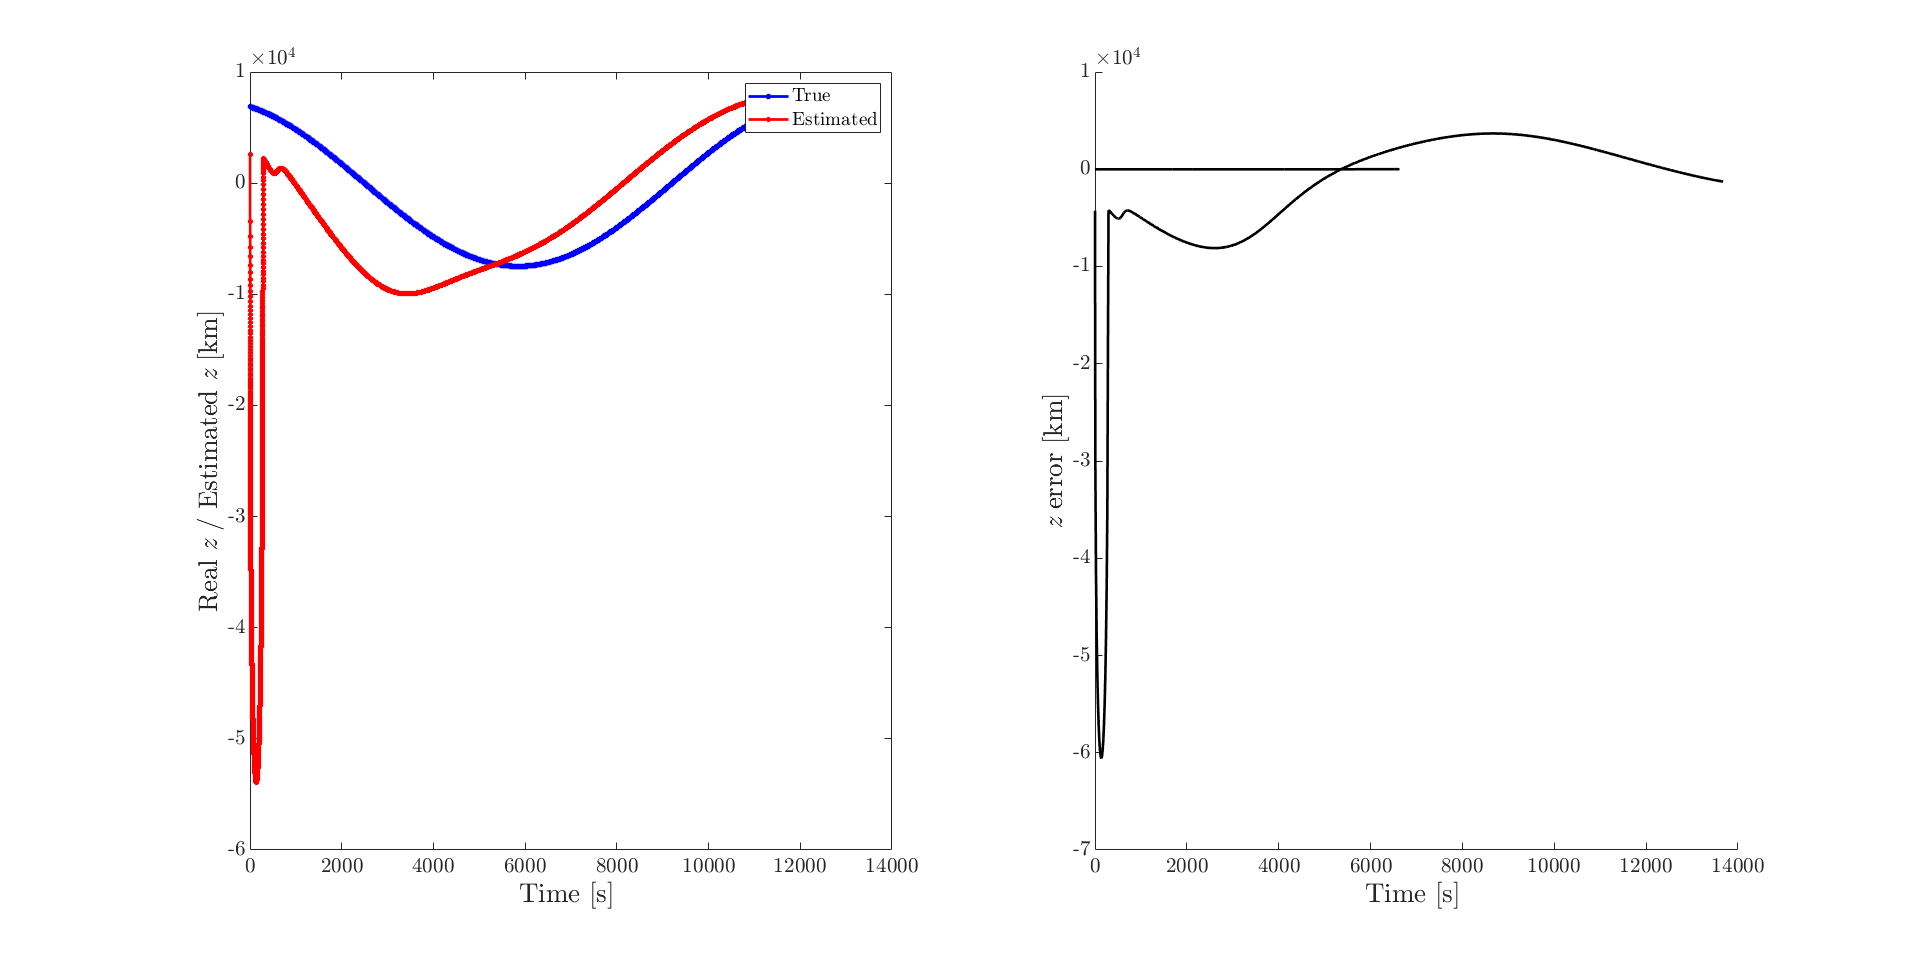
\includegraphics[width=\textwidth]{Figures/z-error-1observers-250km.png}
    \caption{}
    \label{fig: zerror-250-1}
\end{figure}
\begin{figure}[H]
    \centering
    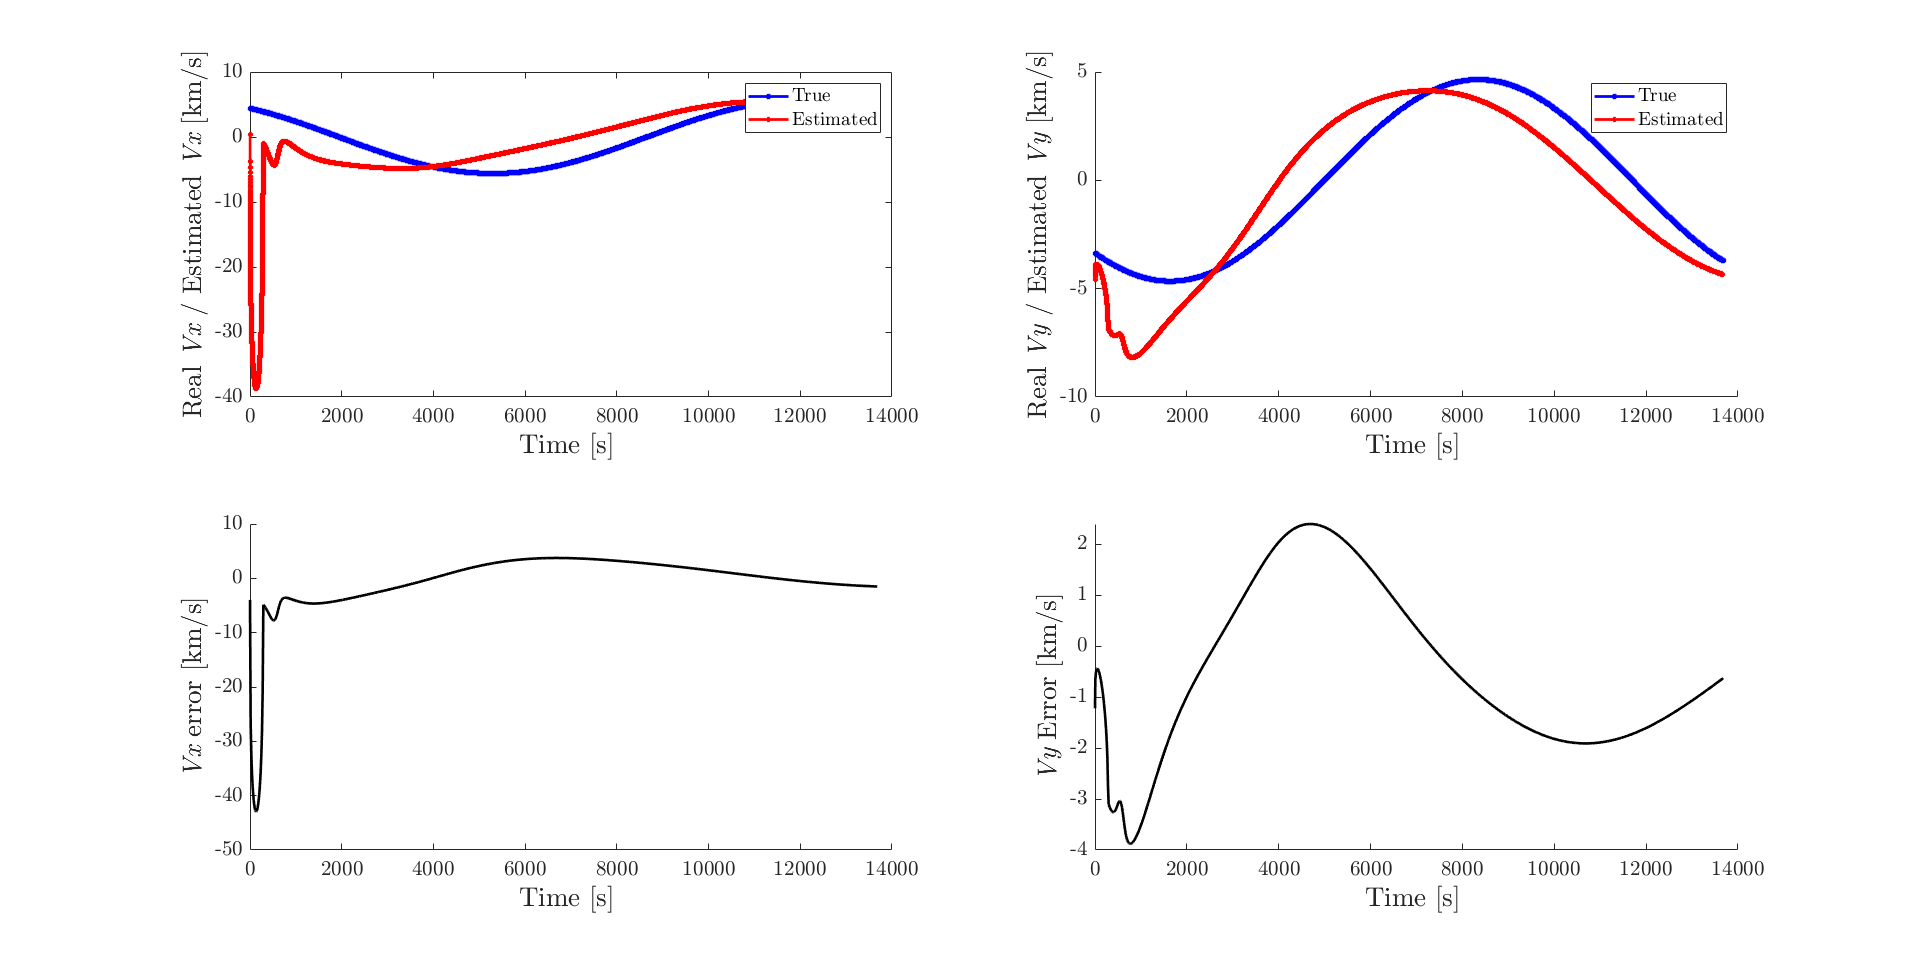
\includegraphics[width=\textwidth]{Figures/Vx-vy-error--250km-1obs.png}
    \caption{}
    \label{fig: vxyerror-250-1}
\end{figure}
\begin{figure}[H]
    \centering
    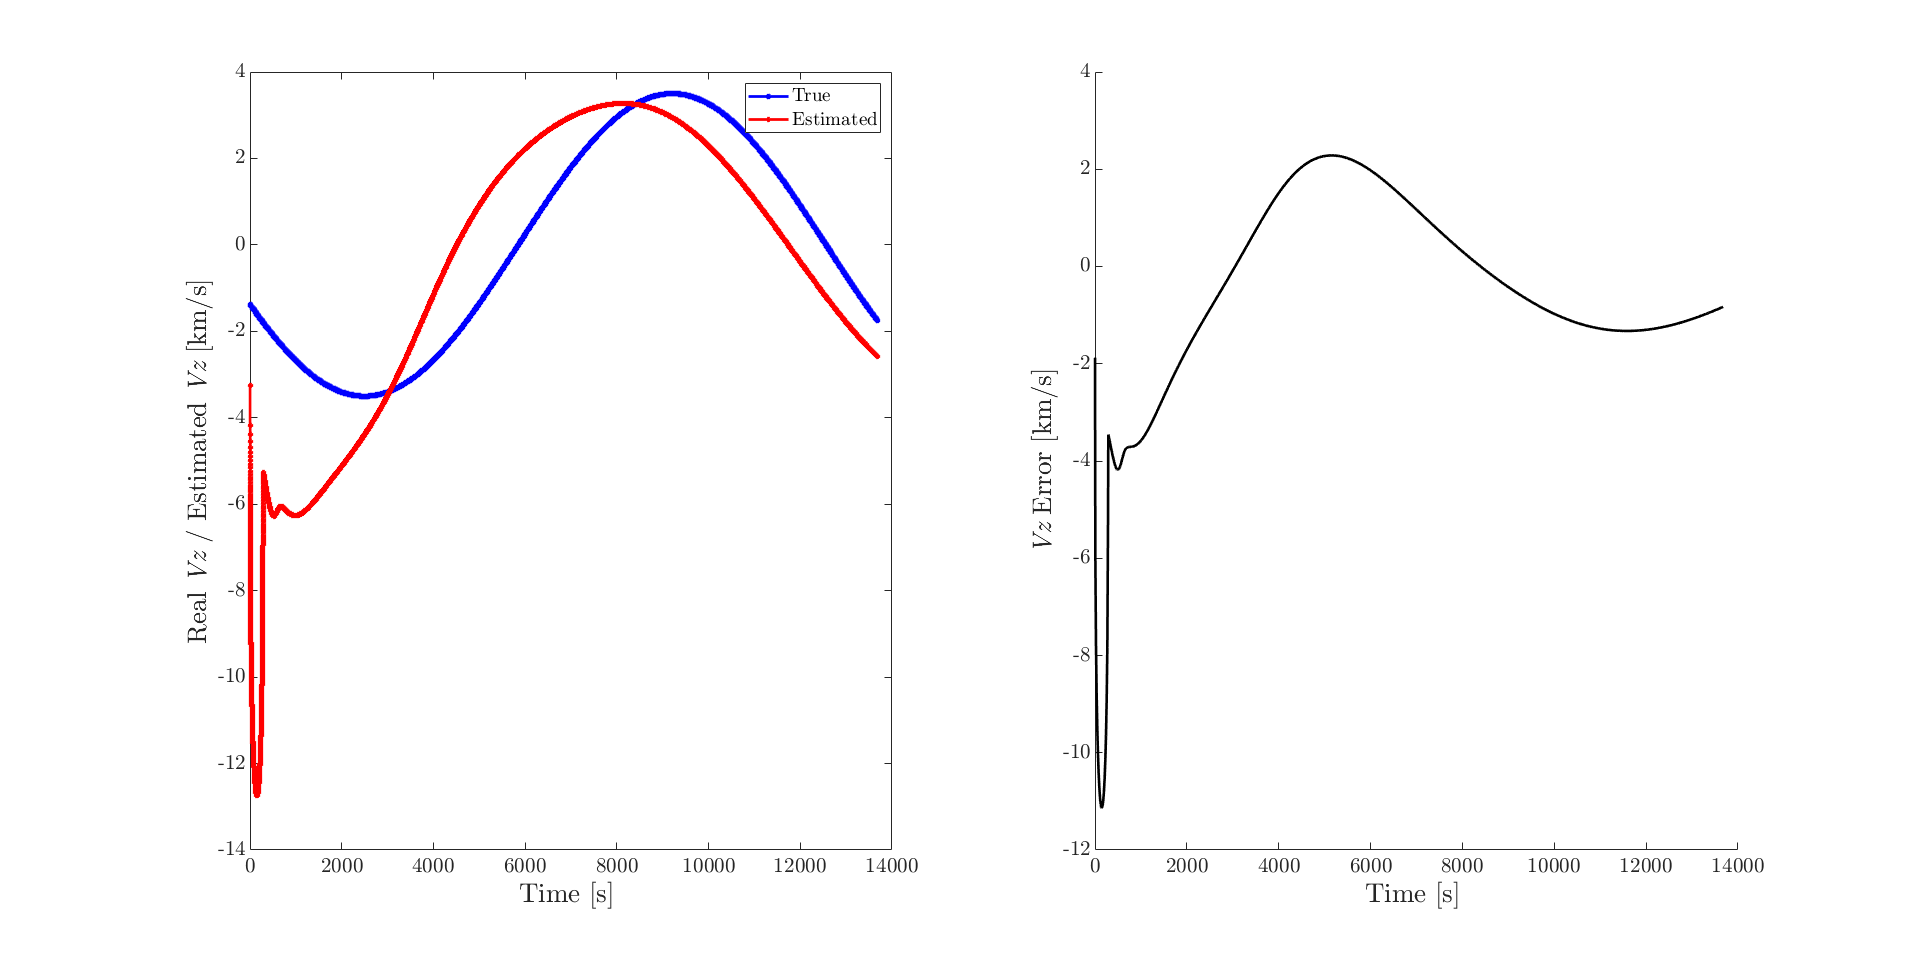
\includegraphics[width=\textwidth]{Figures/VZ_error--250km-1obs.png}
    \caption{}
    \label{fig: vzerror-250-1}
\end{figure}

\begin{figure}[H]
  \begin{subfigure}[b]{0.5\linewidth}
    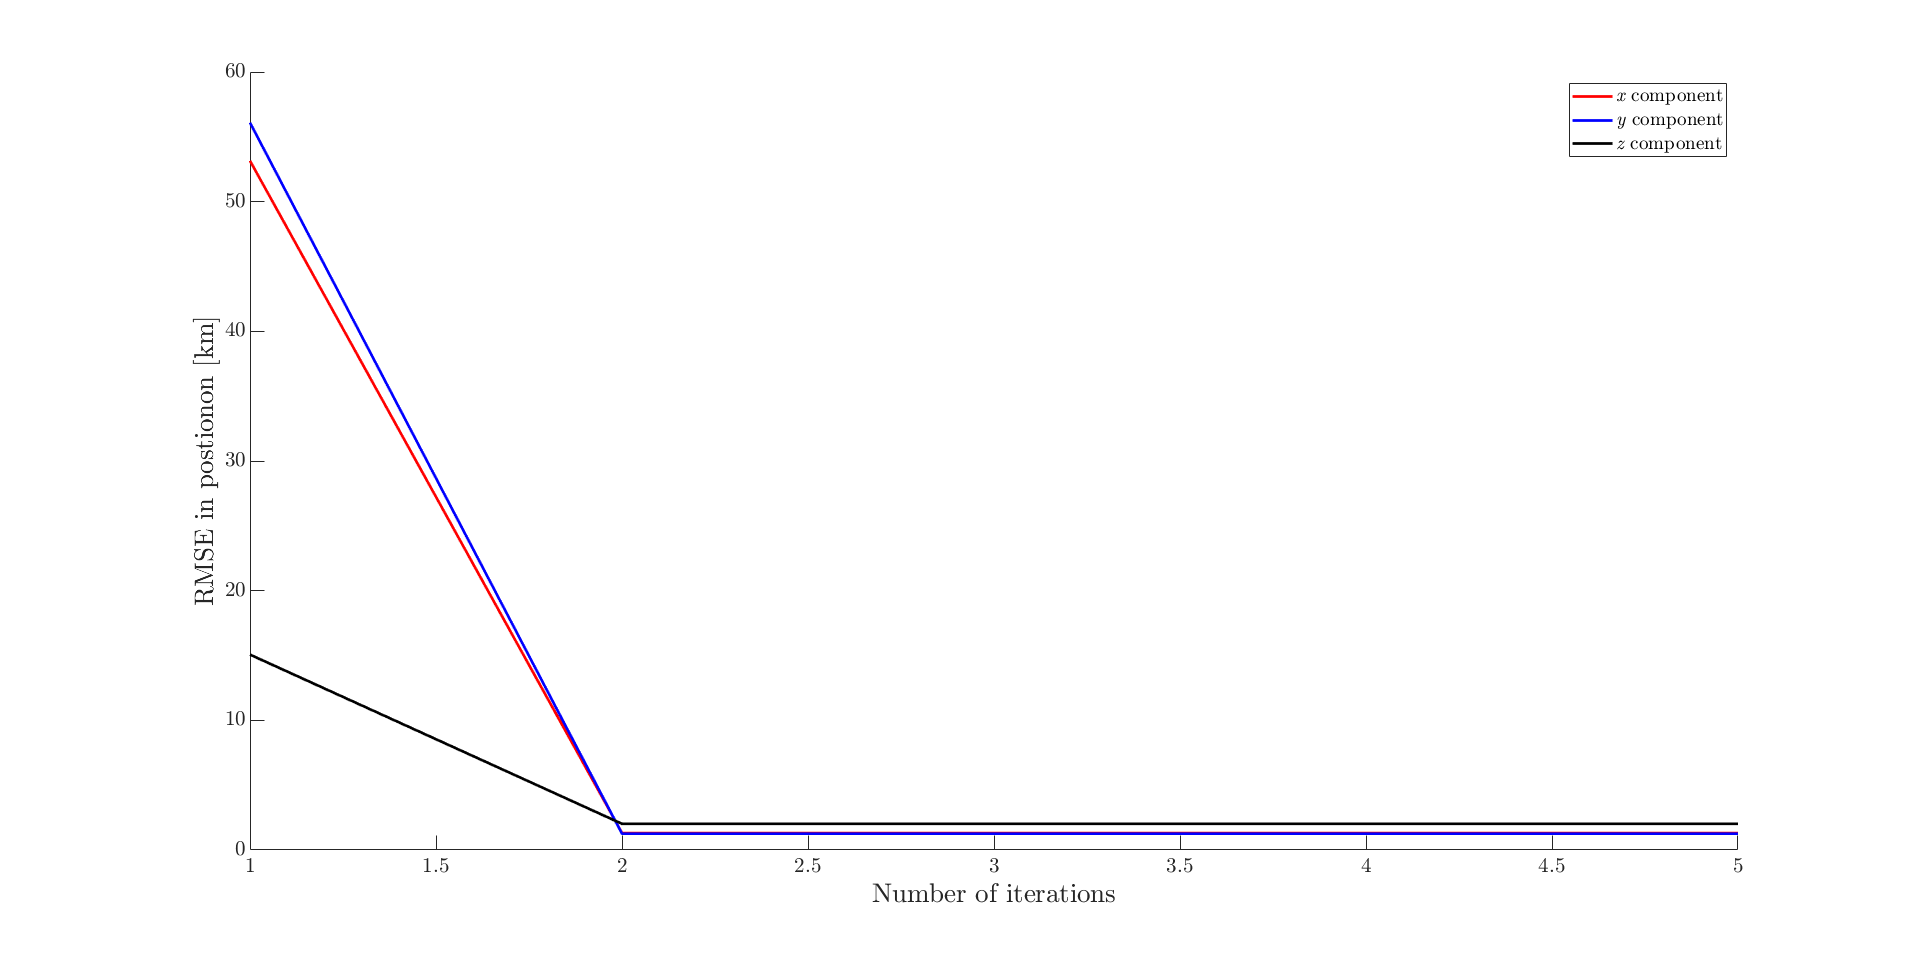
\includegraphics[scale=0.3]{Figures/RMSEvsIterations.png}
    \caption{}
  \end{subfigure}
  \begin{subfigure}[b]{0.5\linewidth}
    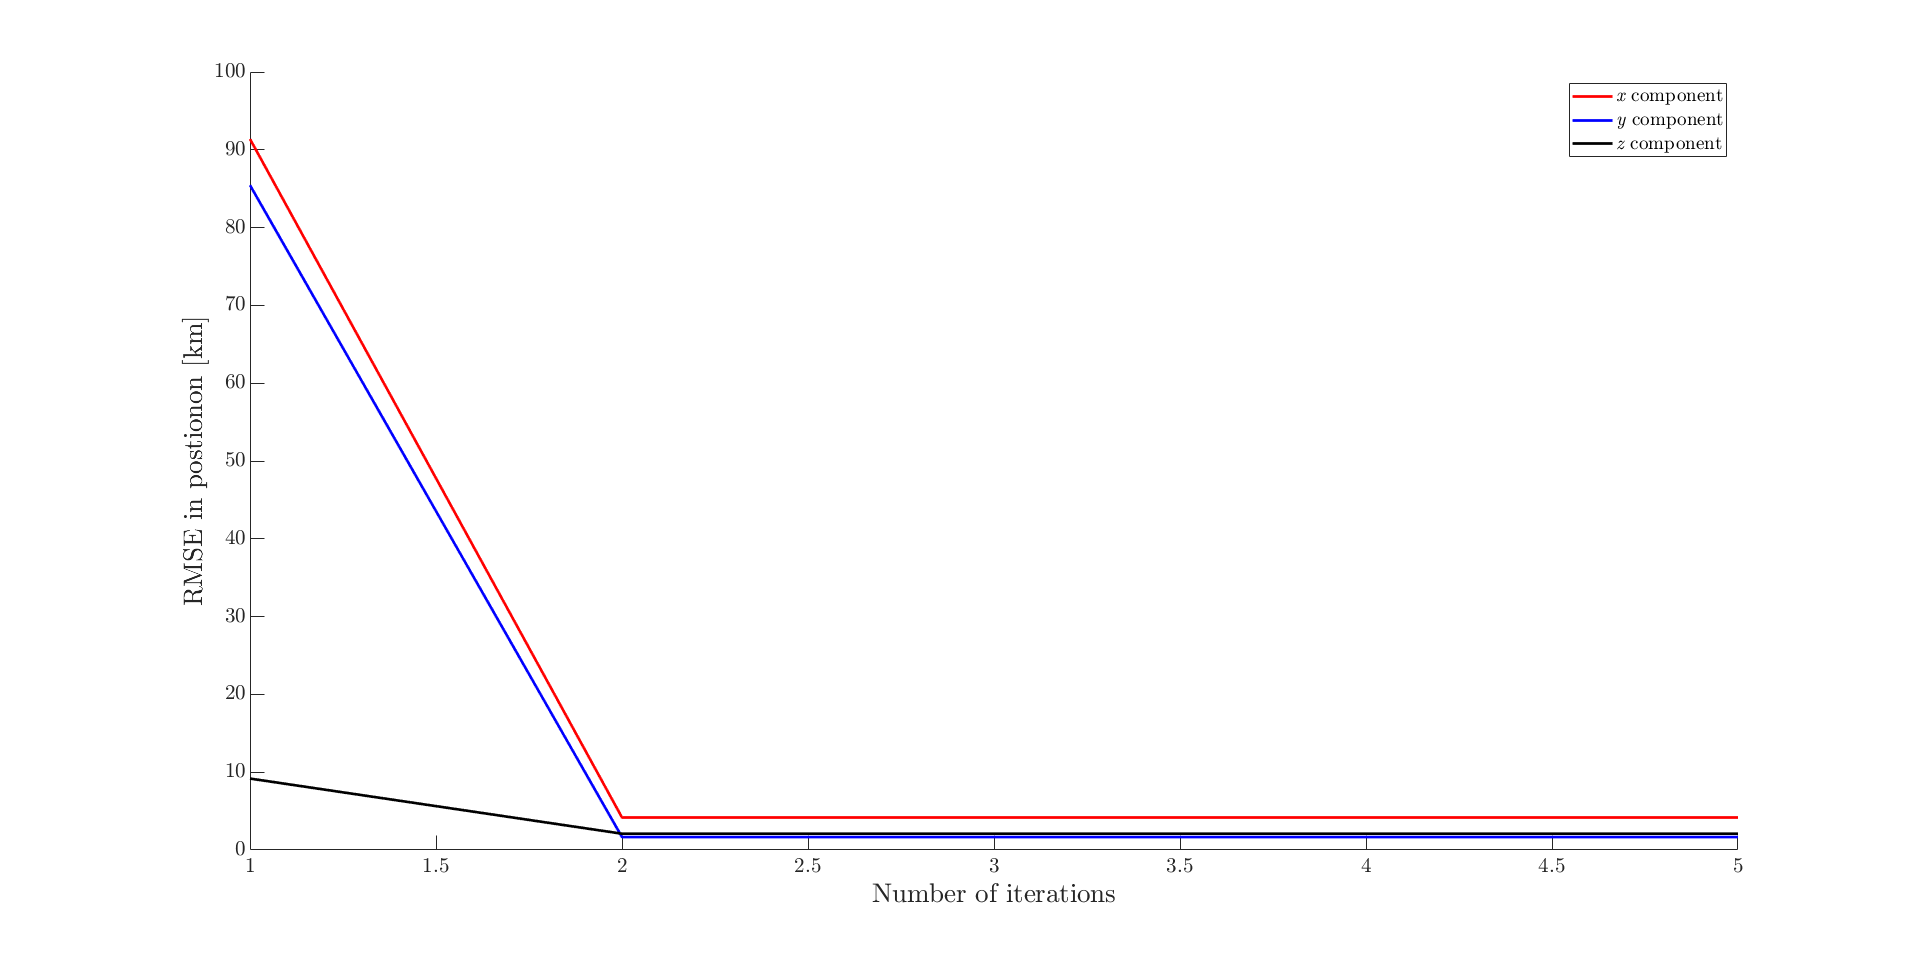
\includegraphics[scale=0.3]{Figures/RMSEvsIterations-5observers-250km.png}
    \caption{}
  \end{subfigure}
  \caption{}
\label{fig: RMSE-5obs}
\end{figure}

\begin{figure}[H]
    \begin{subfigure}[b]{0.5\linewidth}
      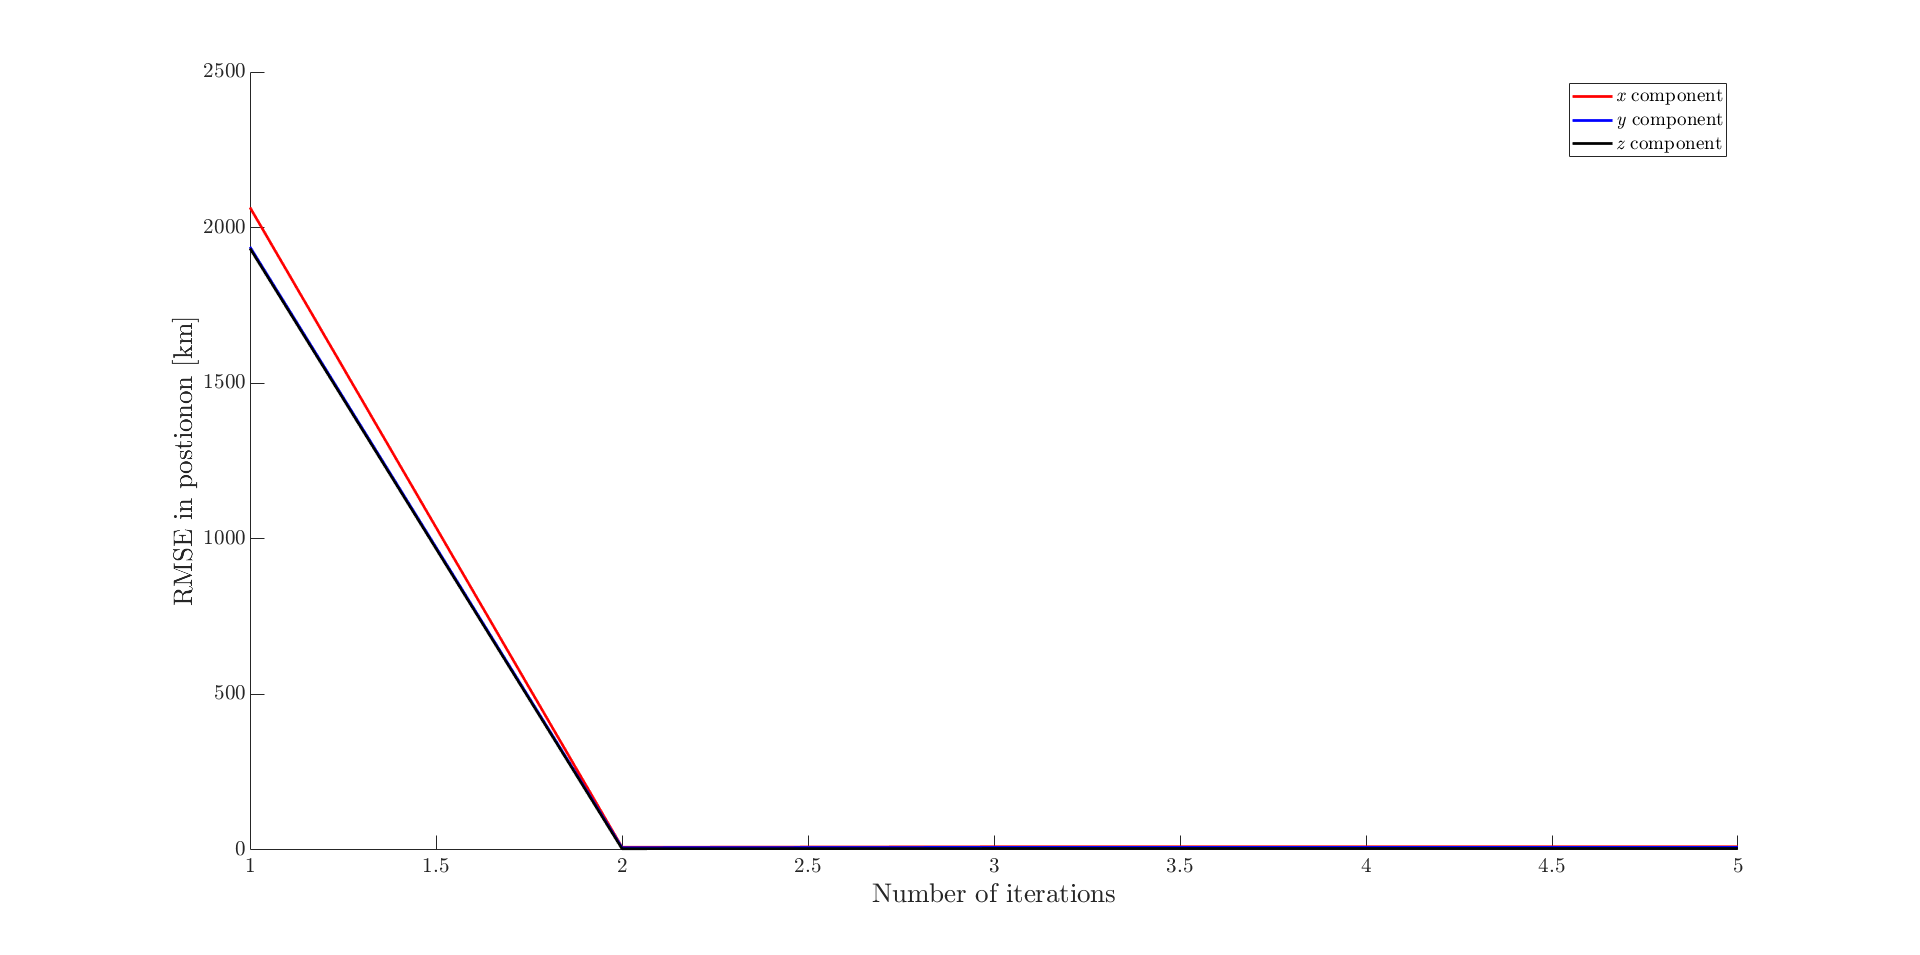
\includegraphics[scale=0.3]{Figures/RMSEvsIterations-50km-1obs.png}
      \caption{}
    \end{subfigure}
    \begin{subfigure}[b]{0.5\linewidth}
      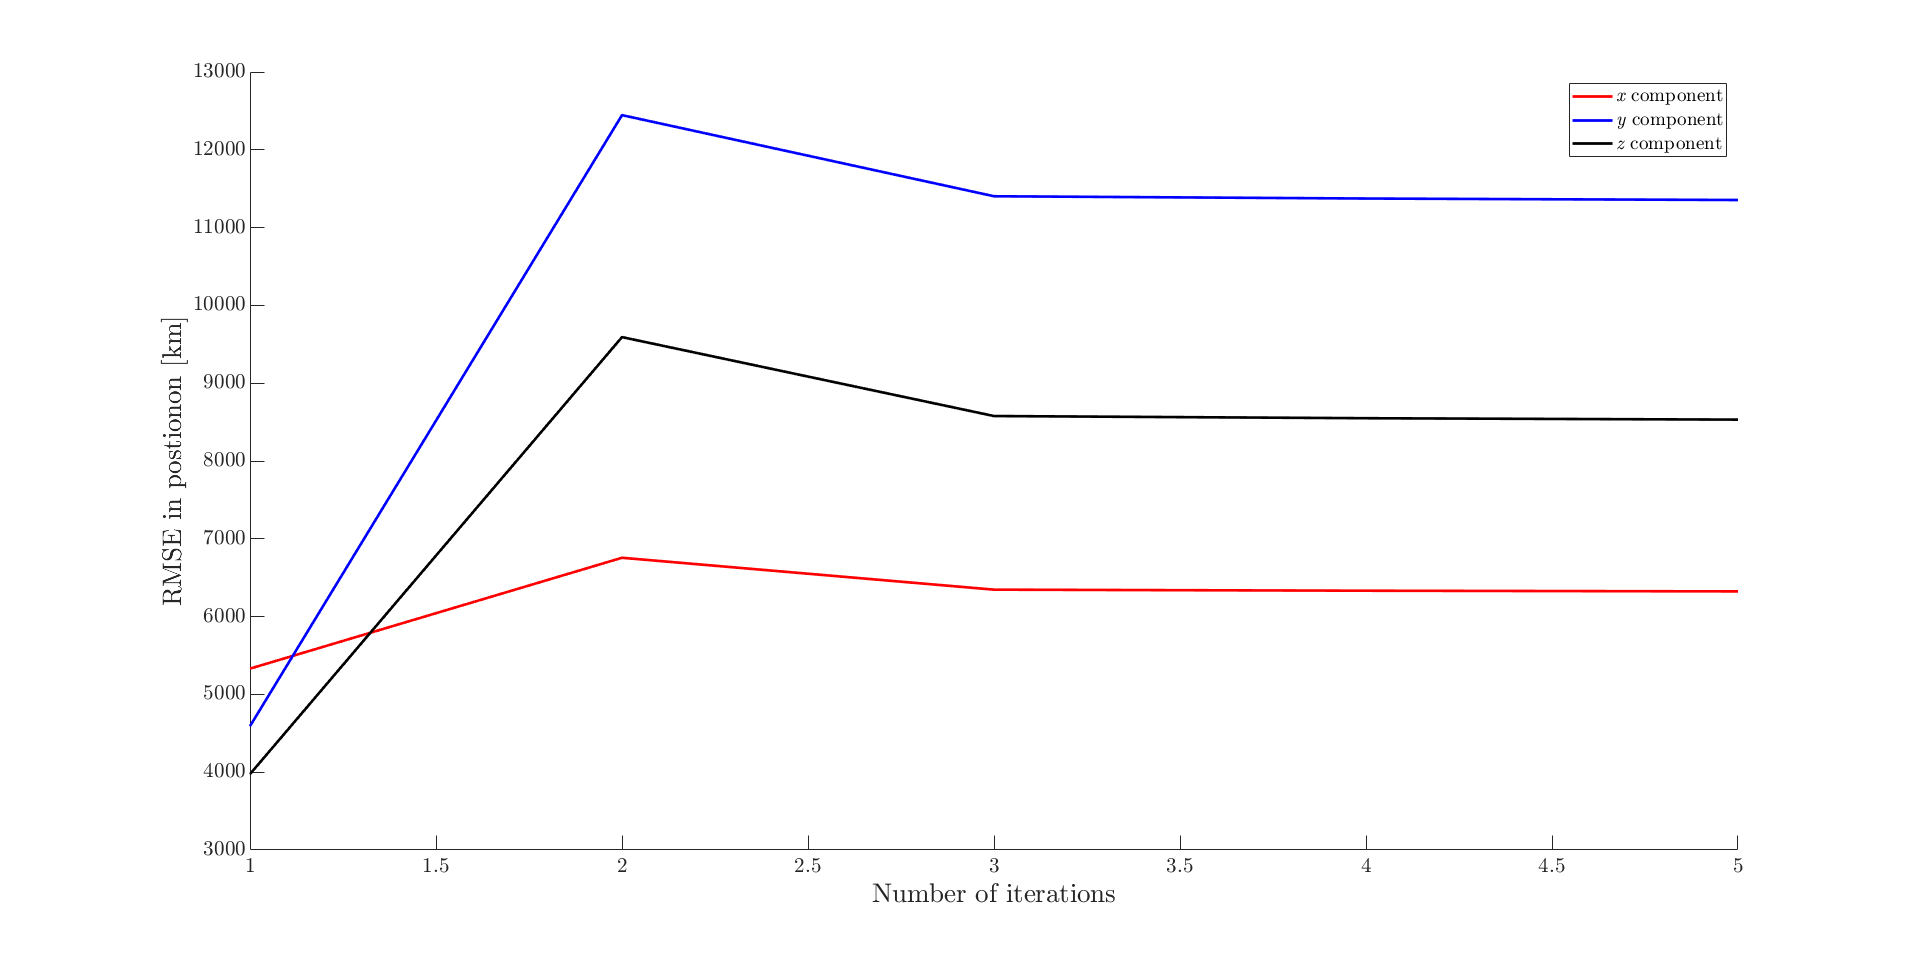
\includegraphics[scale=0.3]{Figures/RMSEvsIterations-250km-1obs.png}
      \caption{}
    \end{subfigure}
    \caption{}
  \label{fig: RMSE-1obs}
  \end{figure}